\section{Results and discussion}
\label{section:4}

\subsection{Variation of global Knudsen number results}
\label{subsection:kn}

\autoref{fig:vcontoursquare} shows the velocity contour around a rounded corner square for varying values of Knudsen number.
\begin{figure}
    \centering
    \begin{subfigure}{0.32\textwidth}
        \centering
        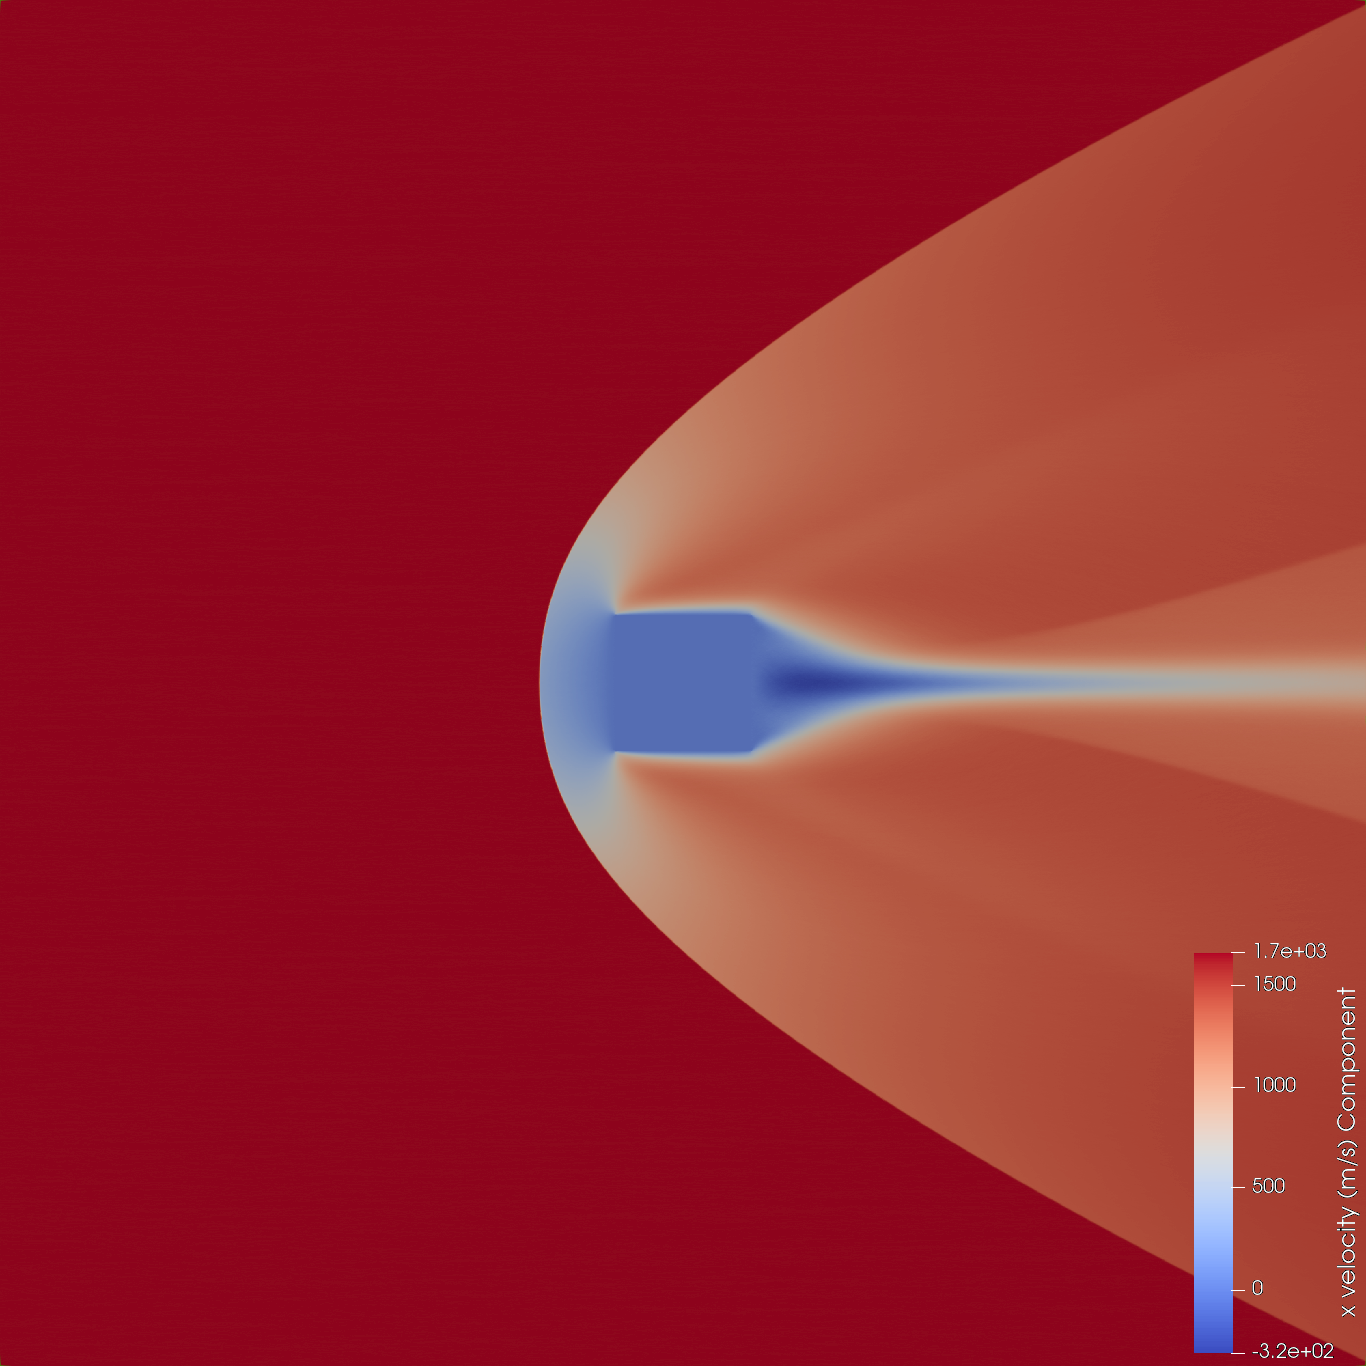
\includegraphics[width=\textwidth]{Images/4. Results/Square Kn/pv/Kn0.001.png}
        \caption{Kn = 0.001}
    \end{subfigure}
    \hfill
    \begin{subfigure}{0.32\textwidth}
        \centering
        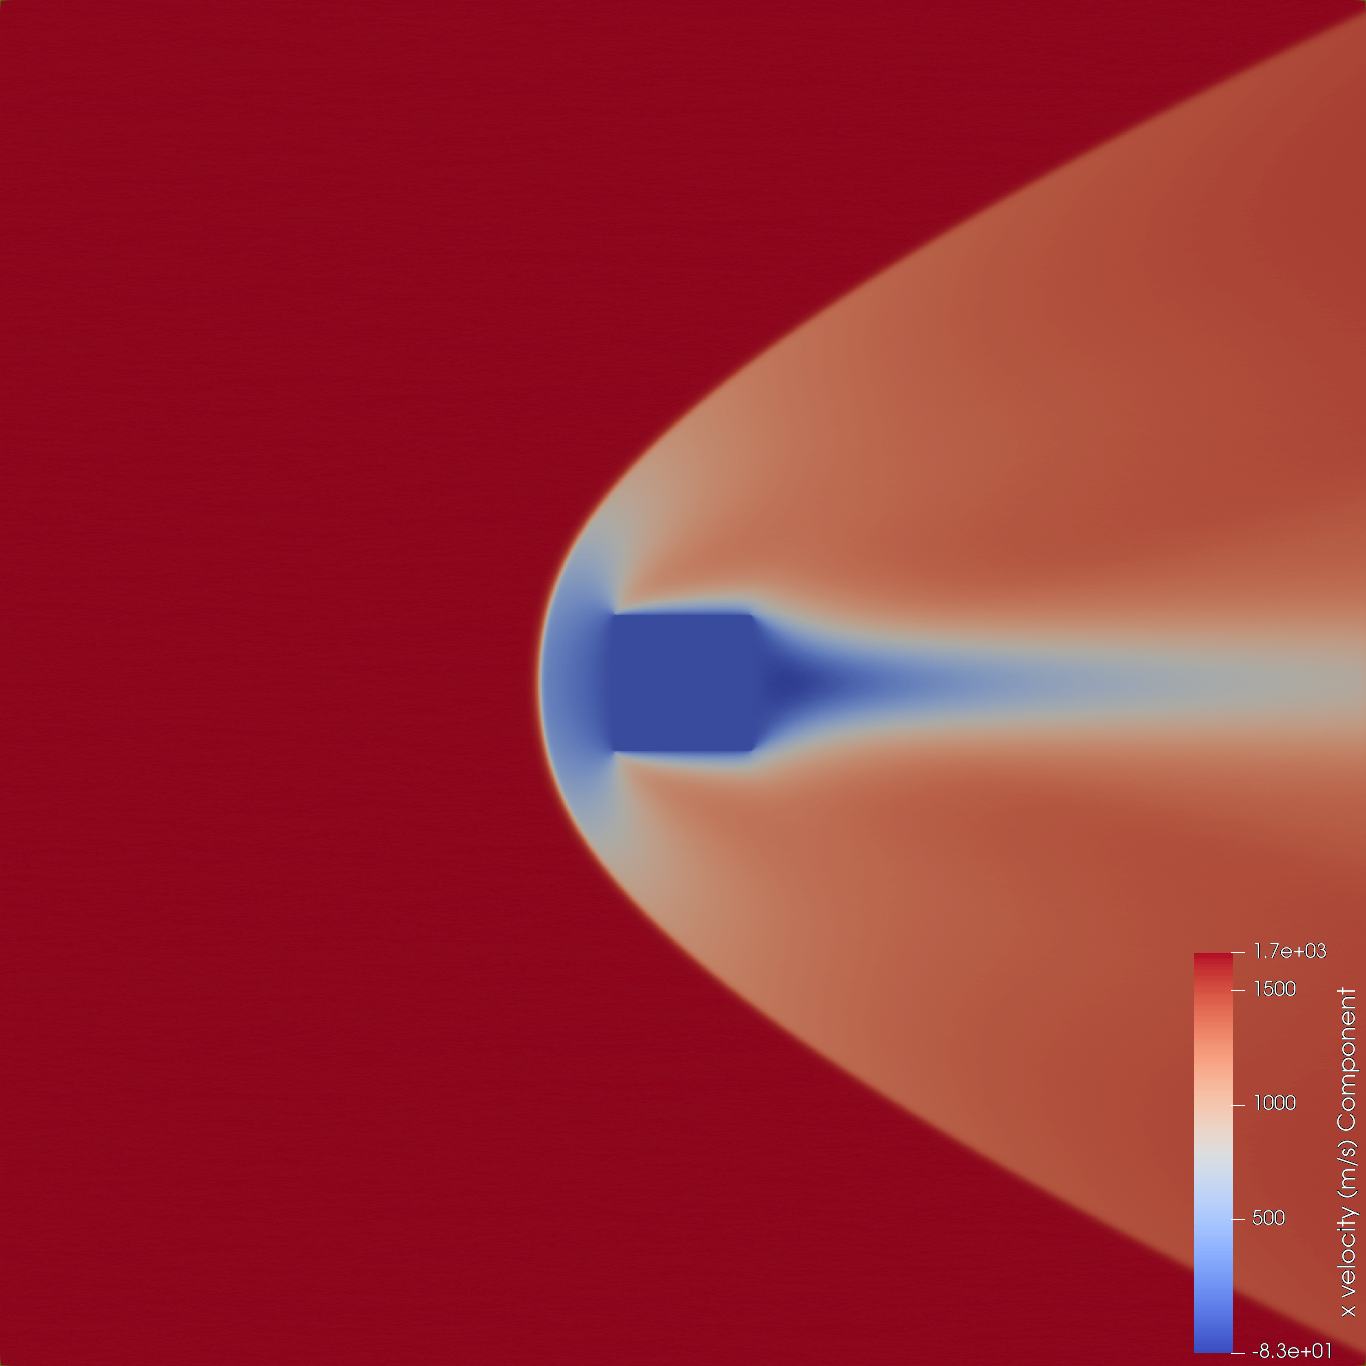
\includegraphics[width=\textwidth]{Images/4. Results/Square Kn/pv/Kn0.01.png}
        \caption{Kn = 0.01}
    \end{subfigure}
    \hfill
    \begin{subfigure}{0.32\textwidth}
        \centering
        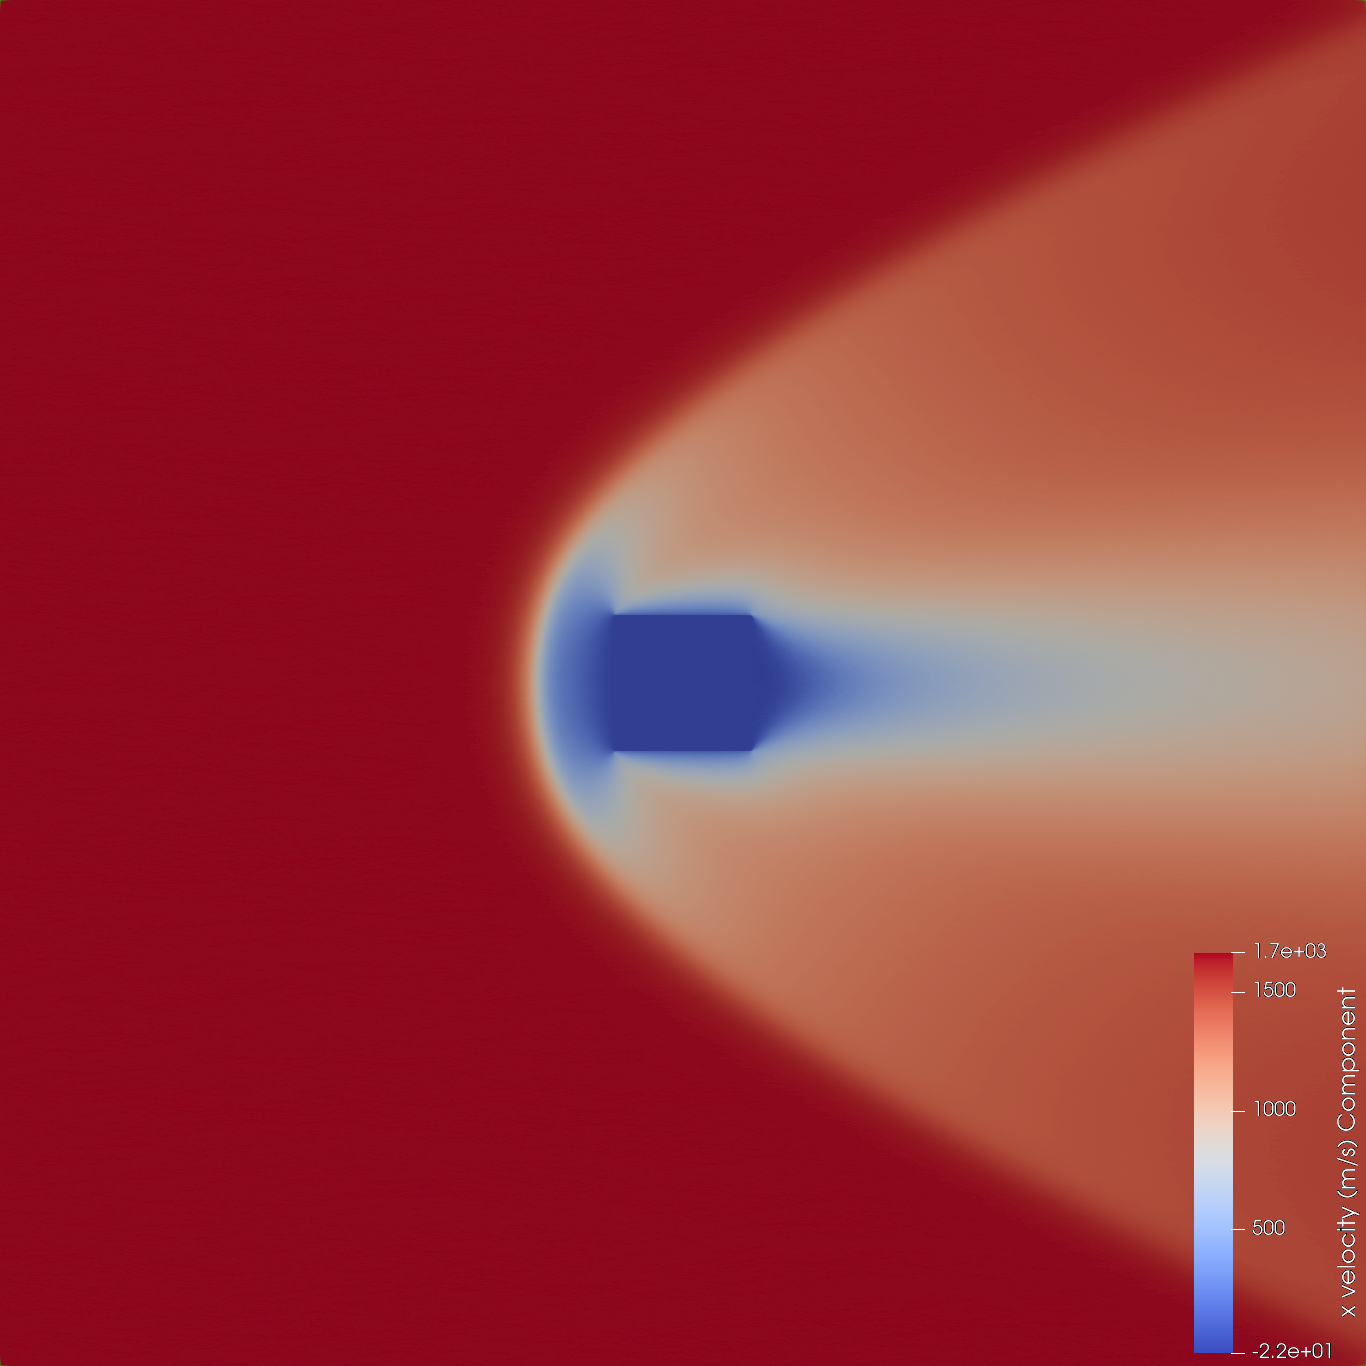
\includegraphics[width=\textwidth]{Images/4. Results/Square Kn/pv/Kn0.05.png}
        \caption{Kn = 0.05}
    \end{subfigure}
    
    \vspace{5pt}
    
    \centering
    \begin{subfigure}{0.32\textwidth}
        \centering
        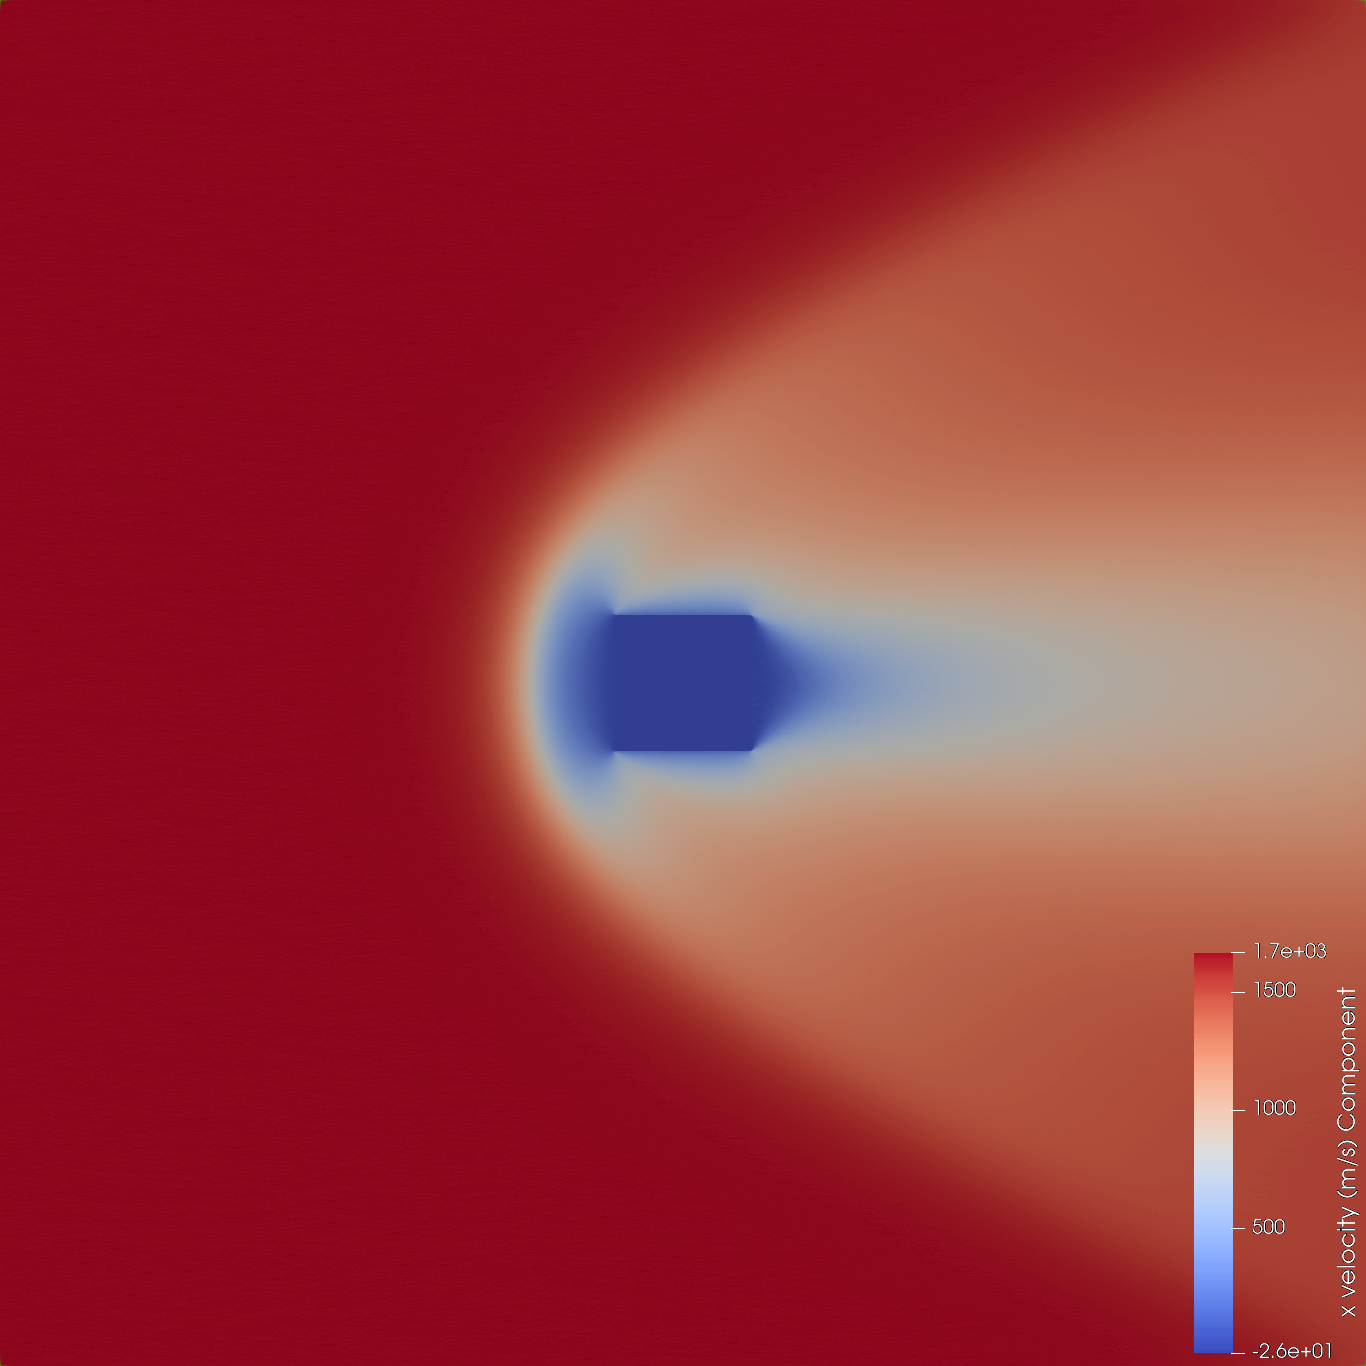
\includegraphics[width=\textwidth]{Images/4. Results/Square Kn/pv/Kn0.1.png}
        \caption{Kn = 0.1}
    \end{subfigure}
    \hfill
    \begin{subfigure}{0.32\textwidth}
        \centering
        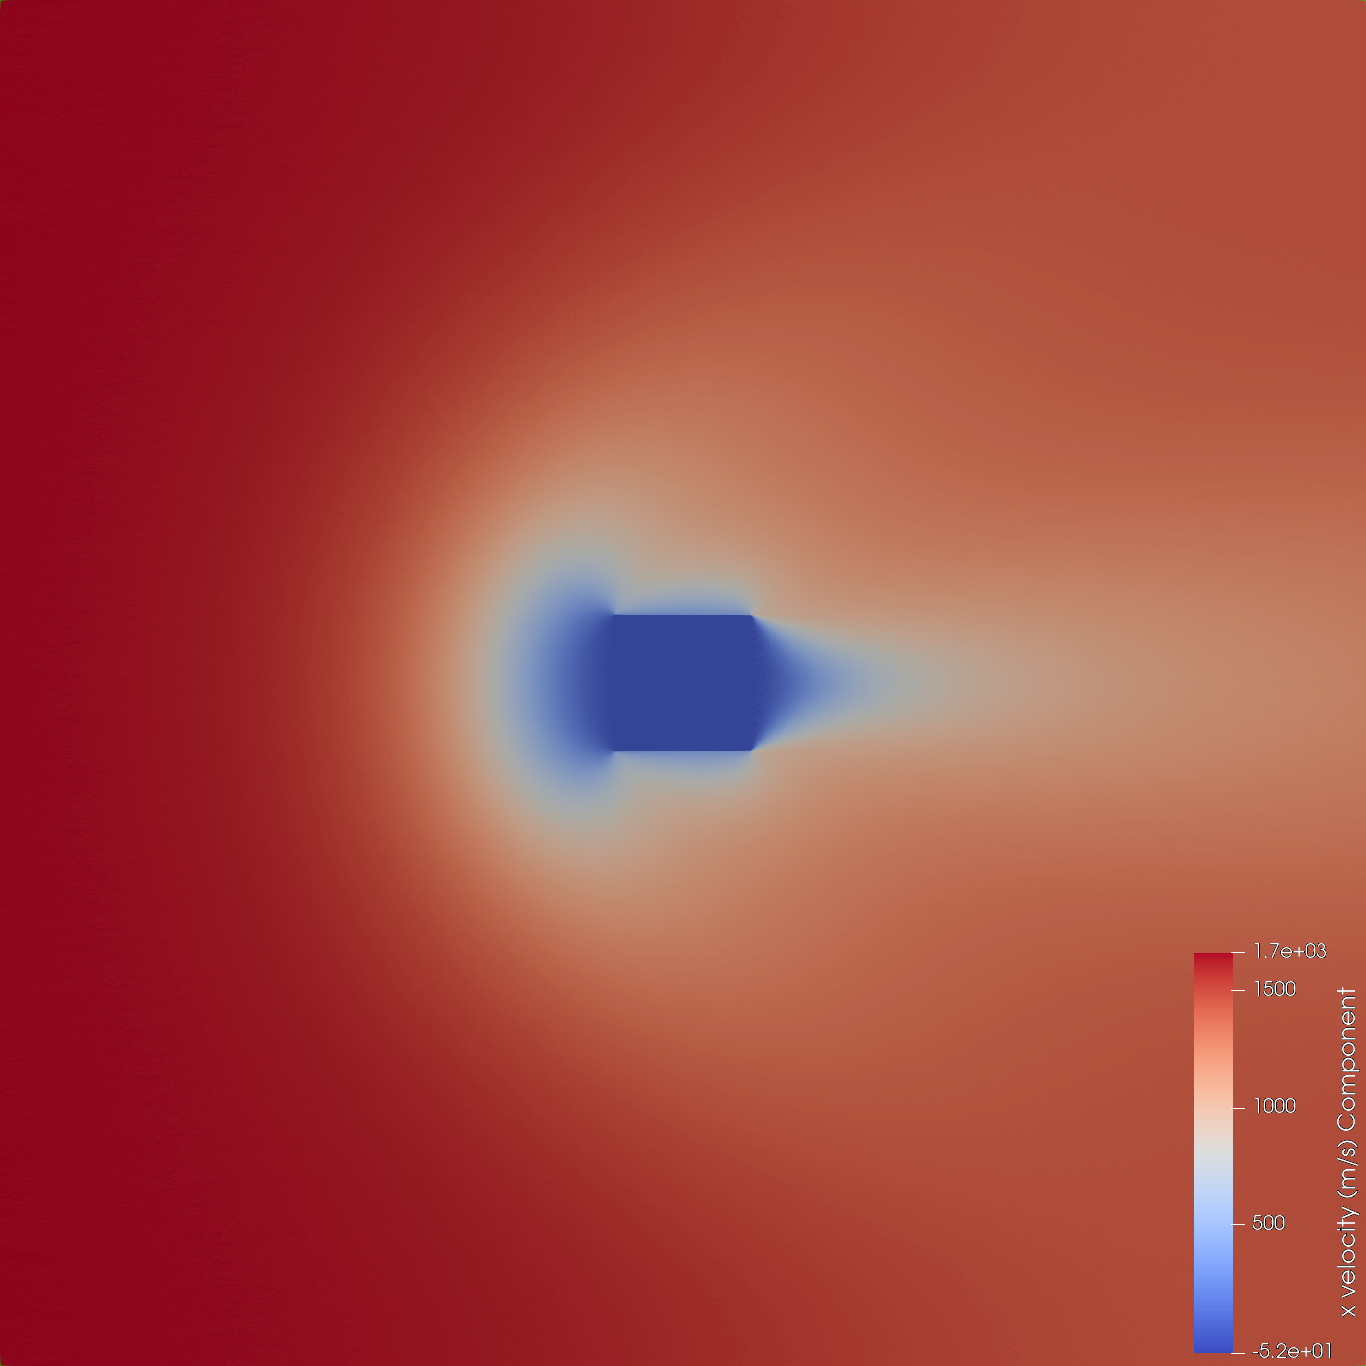
\includegraphics[width=\textwidth]{Images/4. Results/Square Kn/pv/Kn0.5.png}
        \caption{Kn = 0.5}
    \end{subfigure}
    \hfill
    \begin{subfigure}{0.32\textwidth}
        \centering
        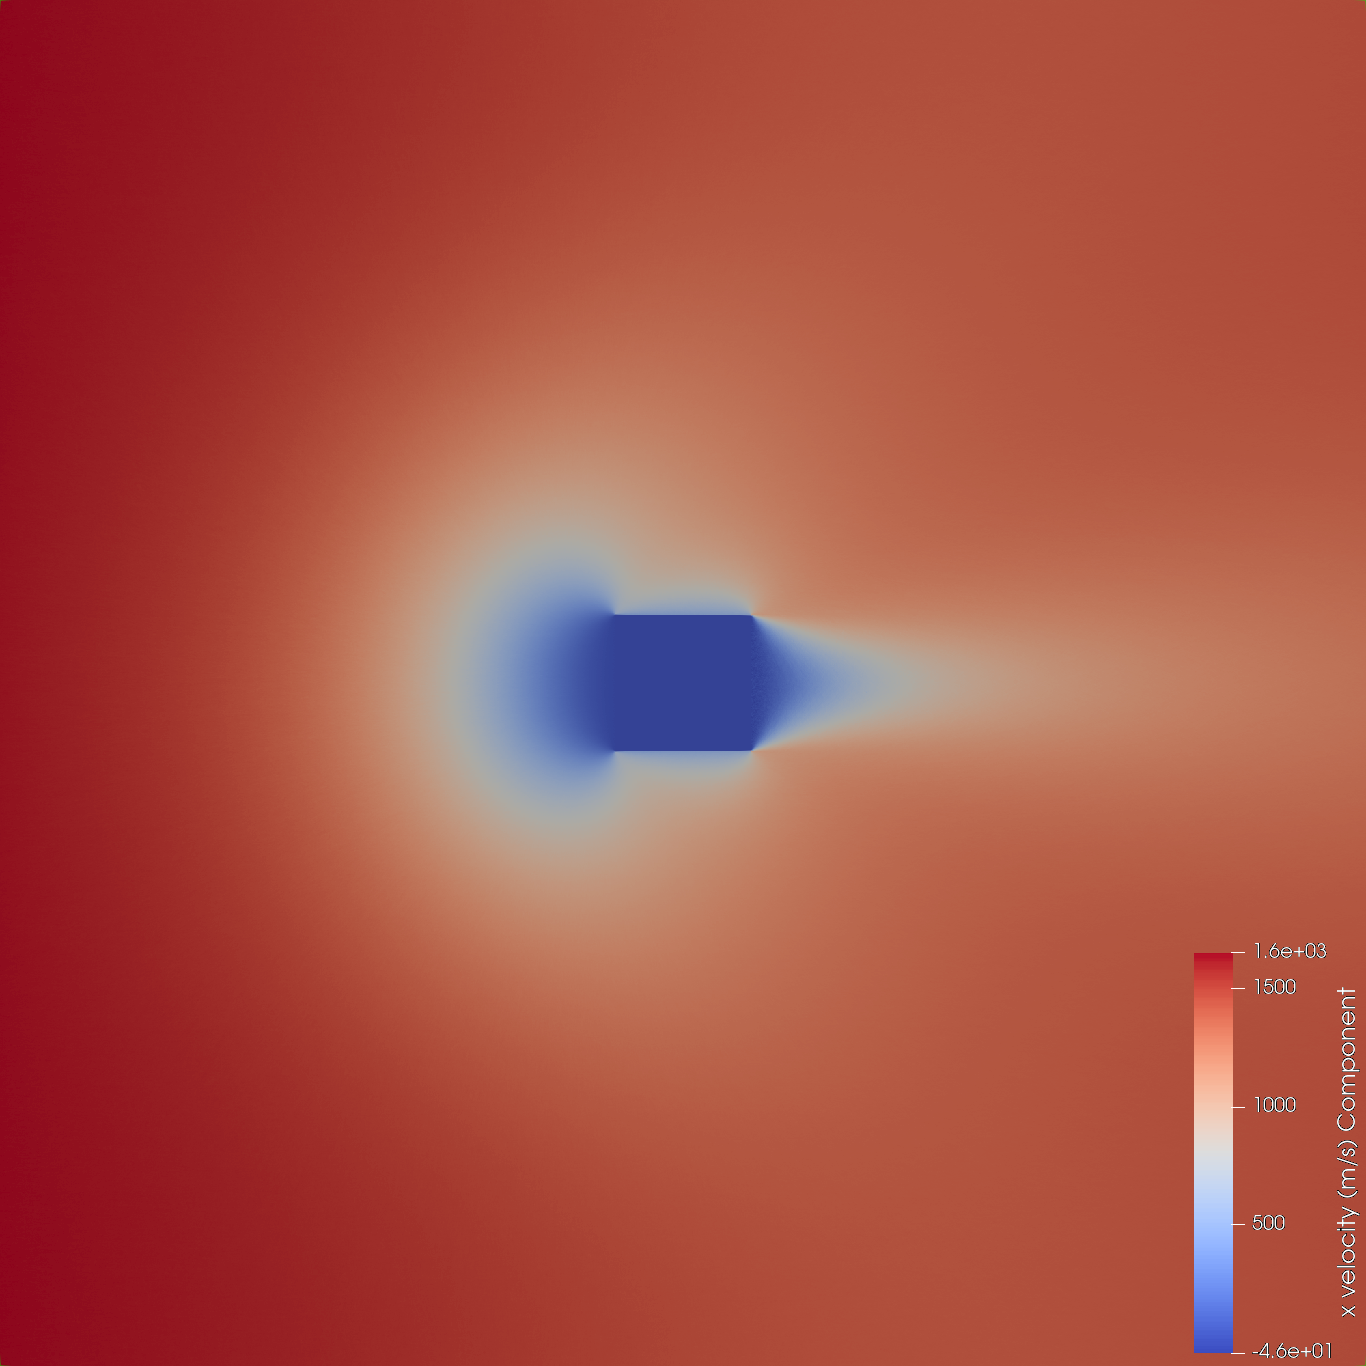
\includegraphics[width=\textwidth]{Images/4. Results/Square Kn/pv/Kn1.png}
        \caption{Kn = 1}
    \end{subfigure}
    
    \vspace{5pt}
    
    \centering
    \begin{subfigure}{0.32\textwidth}
        \centering
        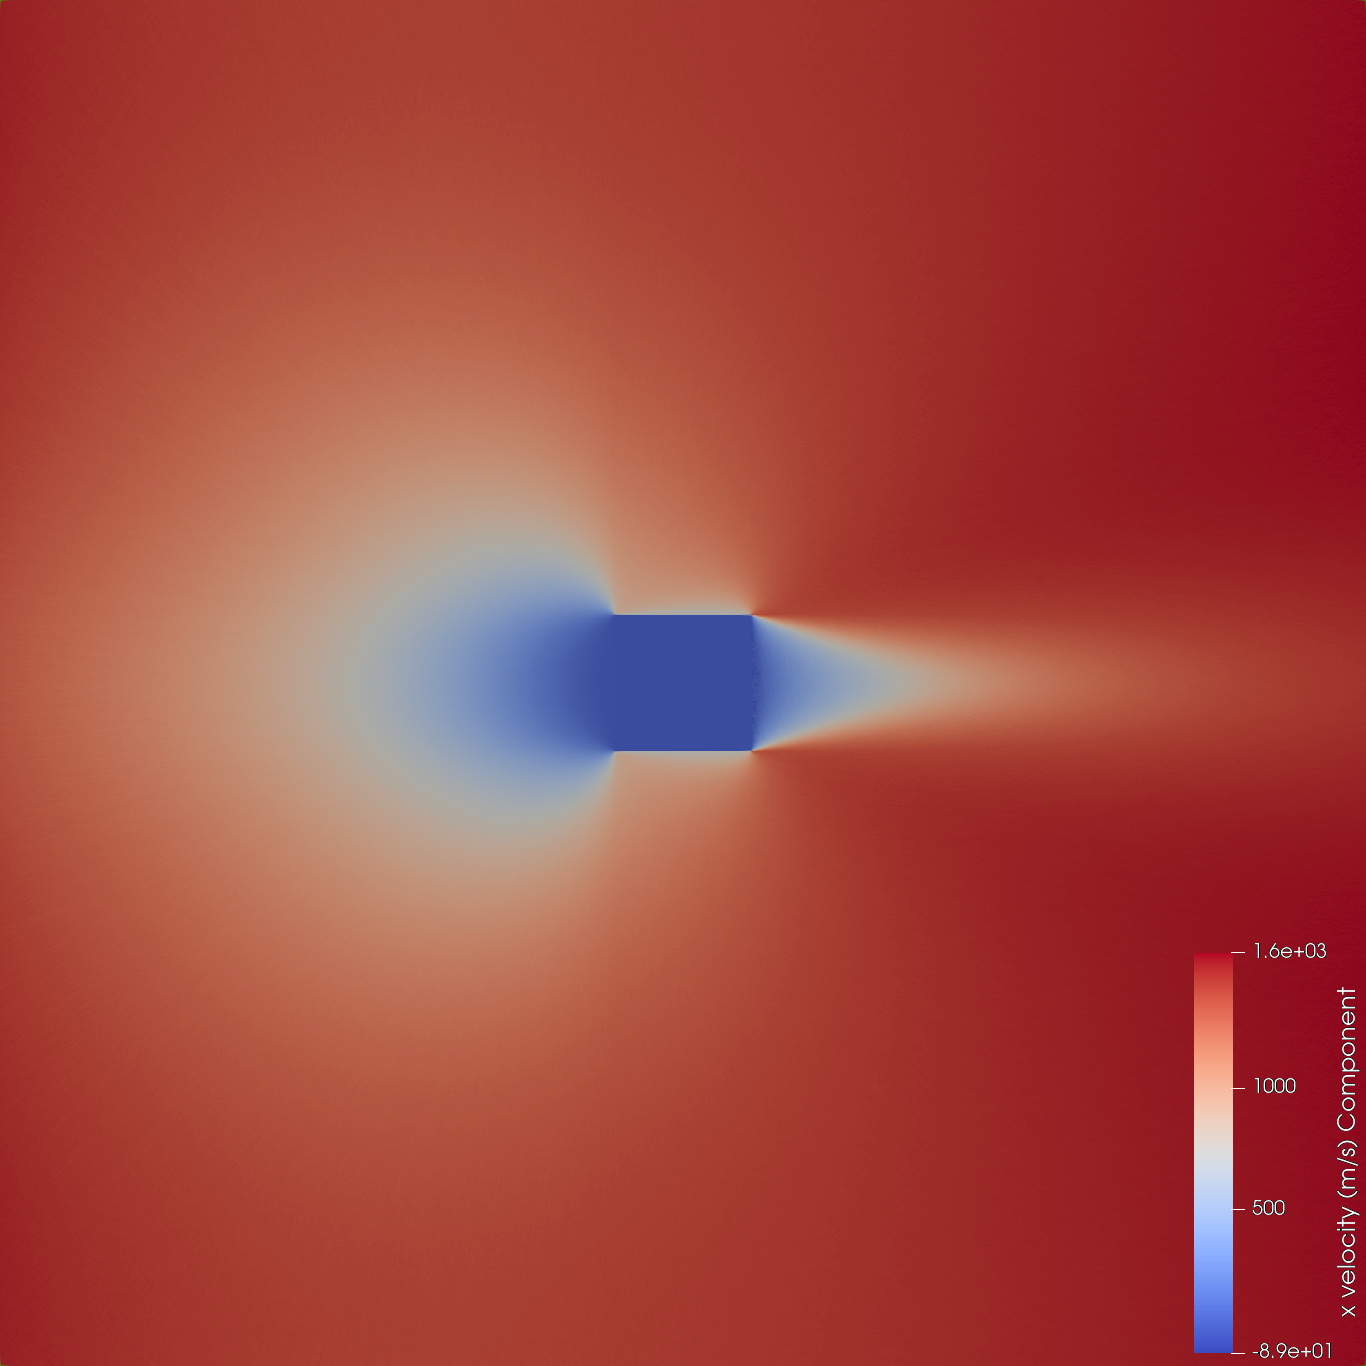
\includegraphics[width=\textwidth]{Images/4. Results/Square Kn/pv/Kn5.png}
        \caption{Kn = 5}
    \end{subfigure}
    \hfill
    \begin{subfigure}{0.32\textwidth}
        \centering
        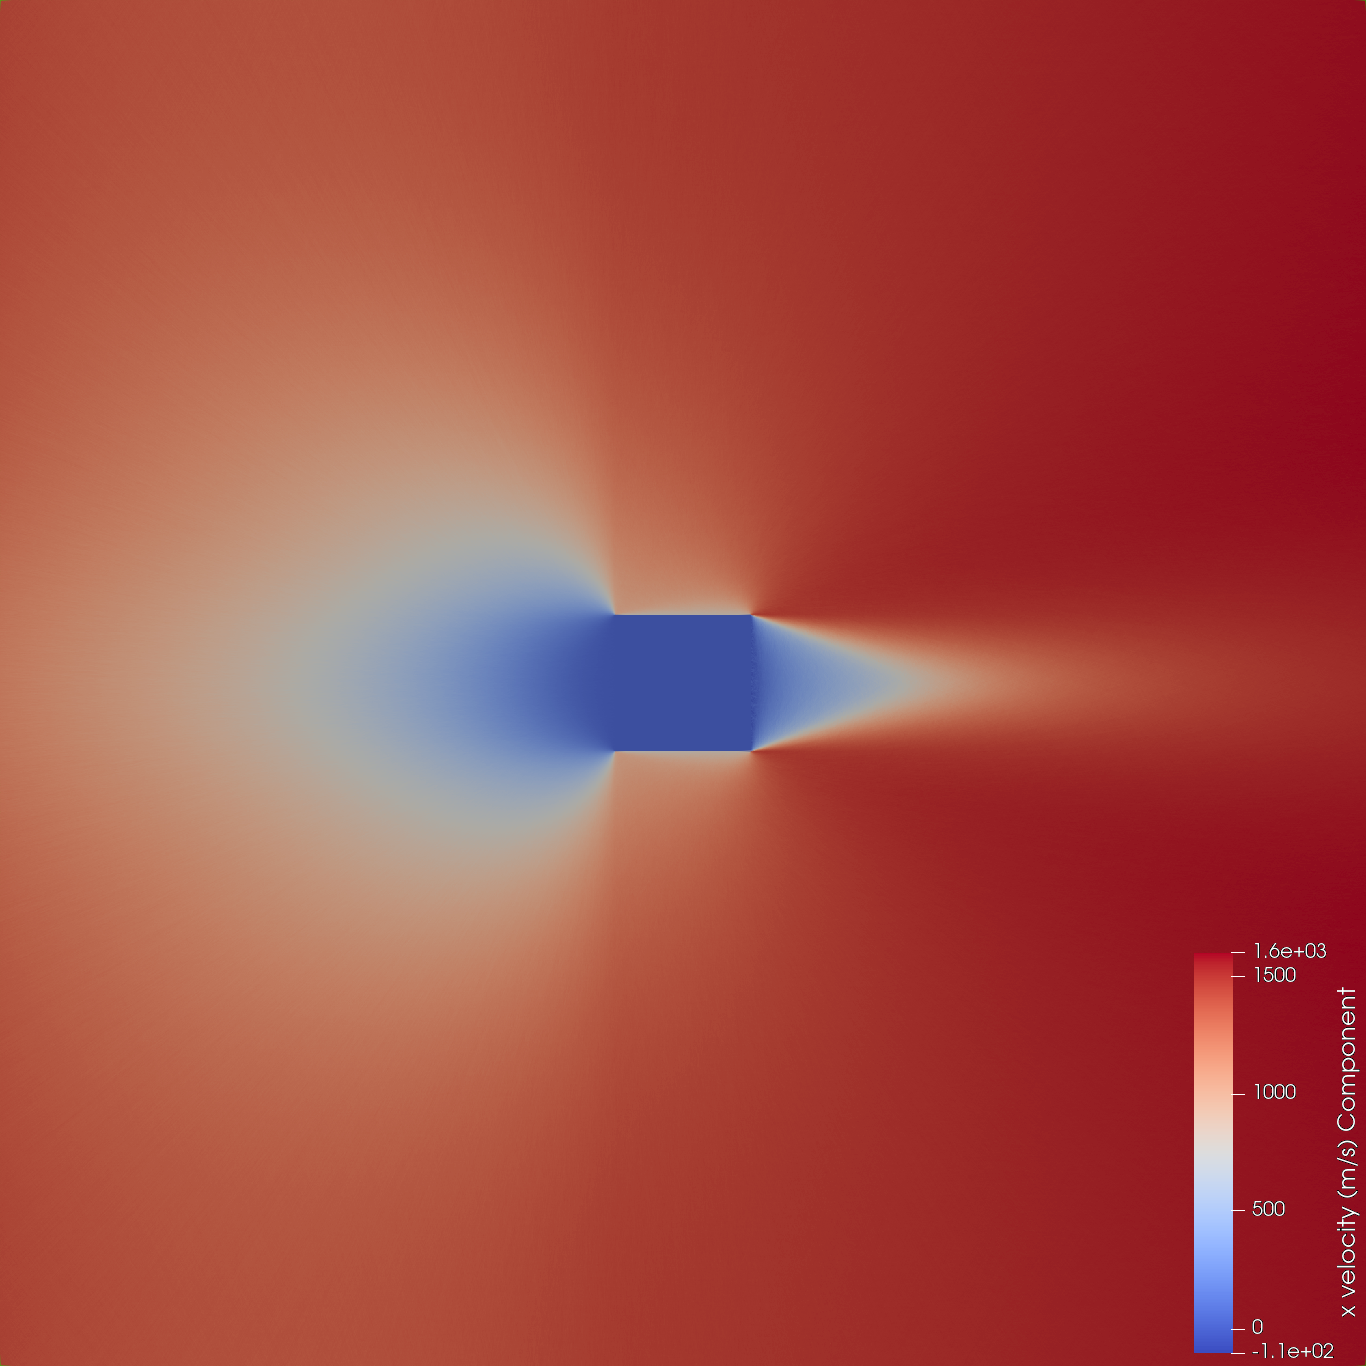
\includegraphics[width=\textwidth]{Images/4. Results/Square Kn/pv/Kn10.png}
        \caption{Kn = 10}
    \end{subfigure}
    \hfill
    \begin{subfigure}{0.32\textwidth}
        \centering
        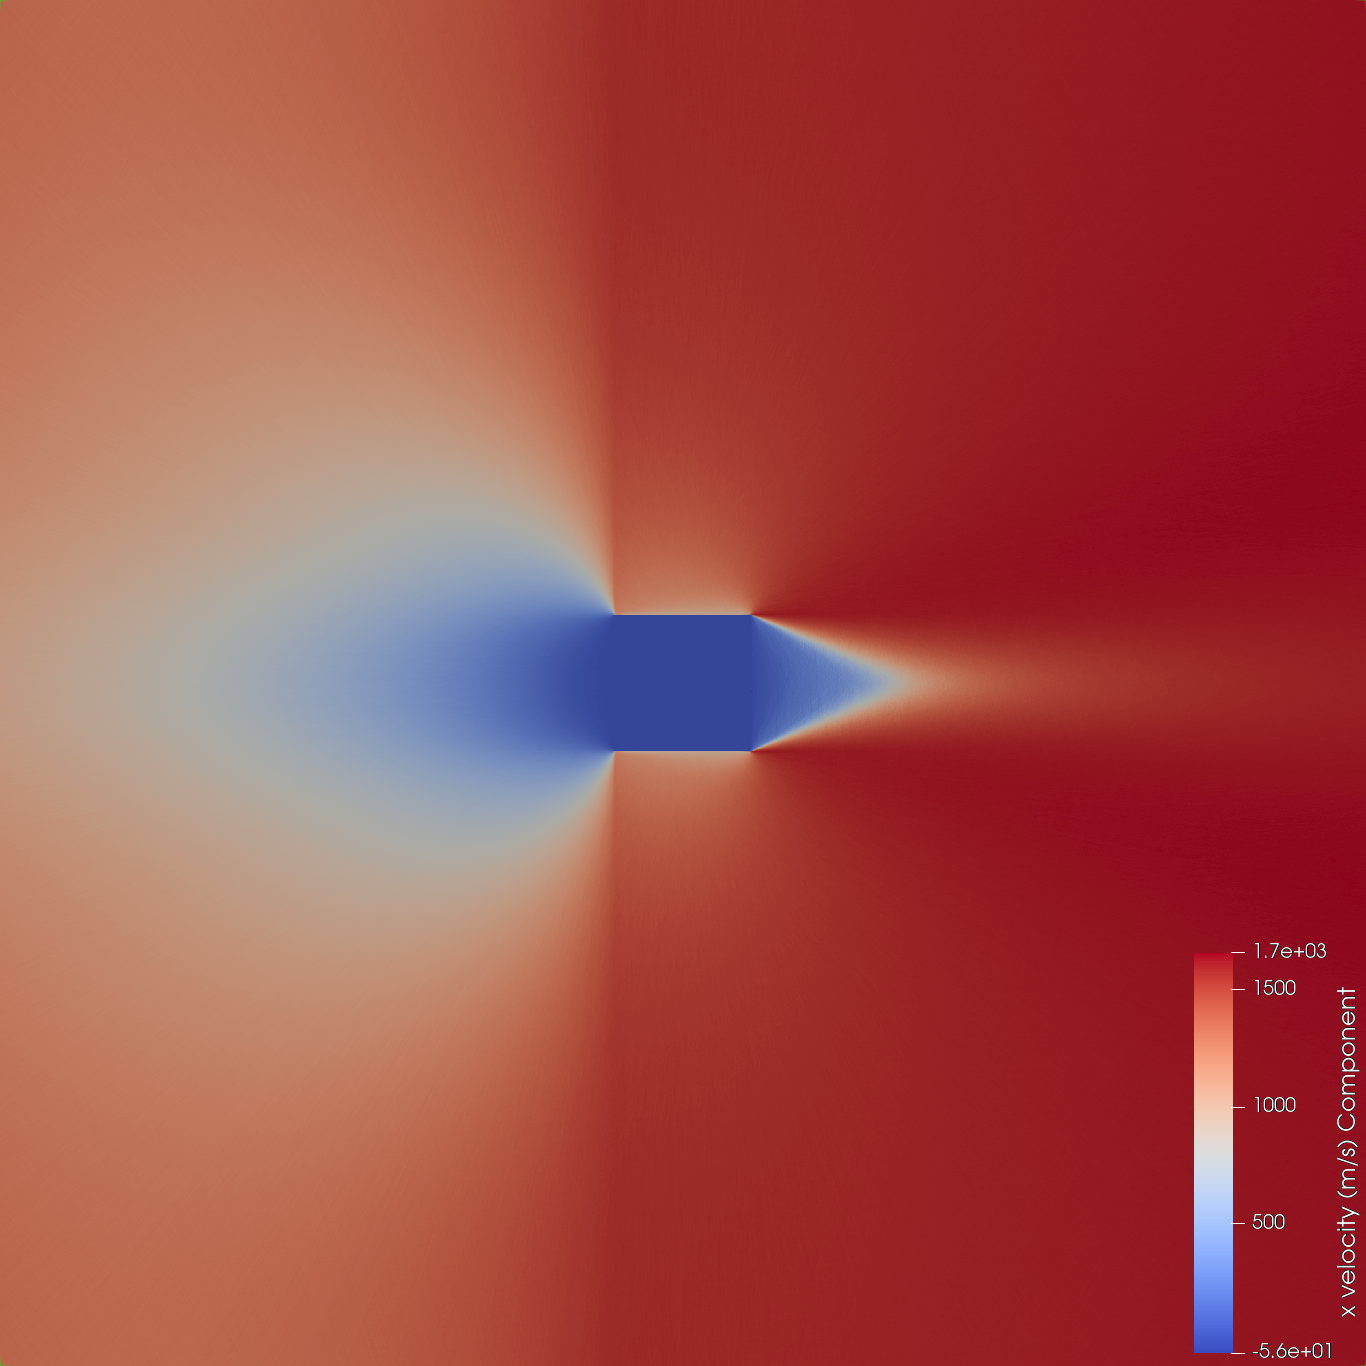
\includegraphics[width=\textwidth]{Images/4. Results/Square Kn/pv/Kn100.png}
        \caption{Kn = 100}
    \end{subfigure}
    \caption{Velocity contours around a rounded square for varying Knudsen number.}
    \label{fig:vcontoursquare}
\end{figure}

A radical change in flow conditions can be observed as the Knudsen number is increased. At a $Kn$ of 0.001, in the pure continuum regime, a number of classical features of supersonic flow can be pointed out: an instantaneous bow shock in front of the cube, expansion fans at its corners and two shocks generated by the expanded flow impinging on itself aft of it. As the Knudsen increased to 0.01 and then to 0.05, a gradual thickening of the boundary layer, typical of a decrease in Reynolds number can be spotted. Moreover, the expansion fans and the shock at the back become gradually less noticeable, and the instantaneous bow shock at the front starts to gradually smear. By $Kn = 0.1$, the shock has become very smeared, and the boundary layer has thickened by a very significant amount. Between the Knudsen numbers of 0.5 and 5, a drastic flow change occurs: the shockwave completely disappears, replaced by a zone of reduced velocity occupying the entire front section of the domain. As Knudsen number is increased even further, this effect becomes more evident, and a peculiar triangular structure (the origin of which his unknown)  appears in the wake of the cube.

This drastic change in flow behaviour could be explained with a paradigm shift in thought process: as mentioned many times, the flow based description of aerodynamics ceases to be valid at high Knudsen number, and it has to be replaced by a particle based one.

In the continuum regime, the flow impinging on the stagnation surface of the cube is forced to curve, first towards the corners and then around them. In a particle sense, when molecules that hit the surface of the cube are reflected in the opposite direction, they encounter other molecules that stop them from travelling against the flow and force them to curve. This produces a bow shock.
However, as the Knudsen number is increased (and thus the density falls), the number of particles forward of those that have just reflected off the surface decreases. Thus, a greater distance is necessary for particles travelling in the opposite direction to be redirected. This can be seen from \autoref{fig:pcontoursquare}.

At very high Knudsen numbers the "stopping effect" disappears almost entirely. Molecules that reflect off the stagnation surface are free to move in the opposite direction, effectively generating a second, completely separate flow.

The reduced velocity magnitude seen in front of the cube is thus probably an artefact, produced by the software as described in \autoref{eq:velocity} by averaging the velocity values of the particles belonging to the two flows over the cell area.

\begin{figure}
    \centering
    \begin{subfigure}{0.32\textwidth}
        \centering
        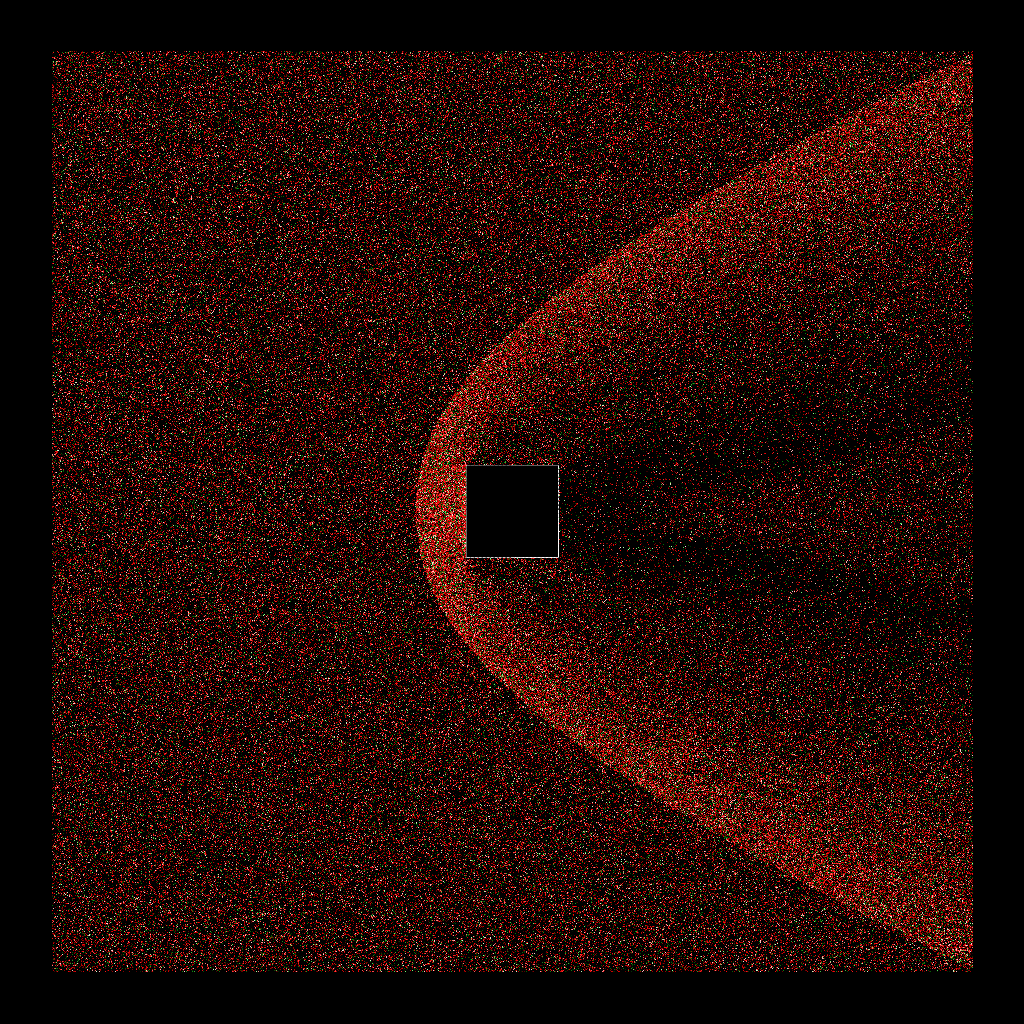
\includegraphics[width=\textwidth]{Images/4. Results/Square Kn/particles/Kn0.001.png}
        \caption{Kn = 0.001}
    \end{subfigure}
    \hfill
    \begin{subfigure}{0.32\textwidth}
        \centering
        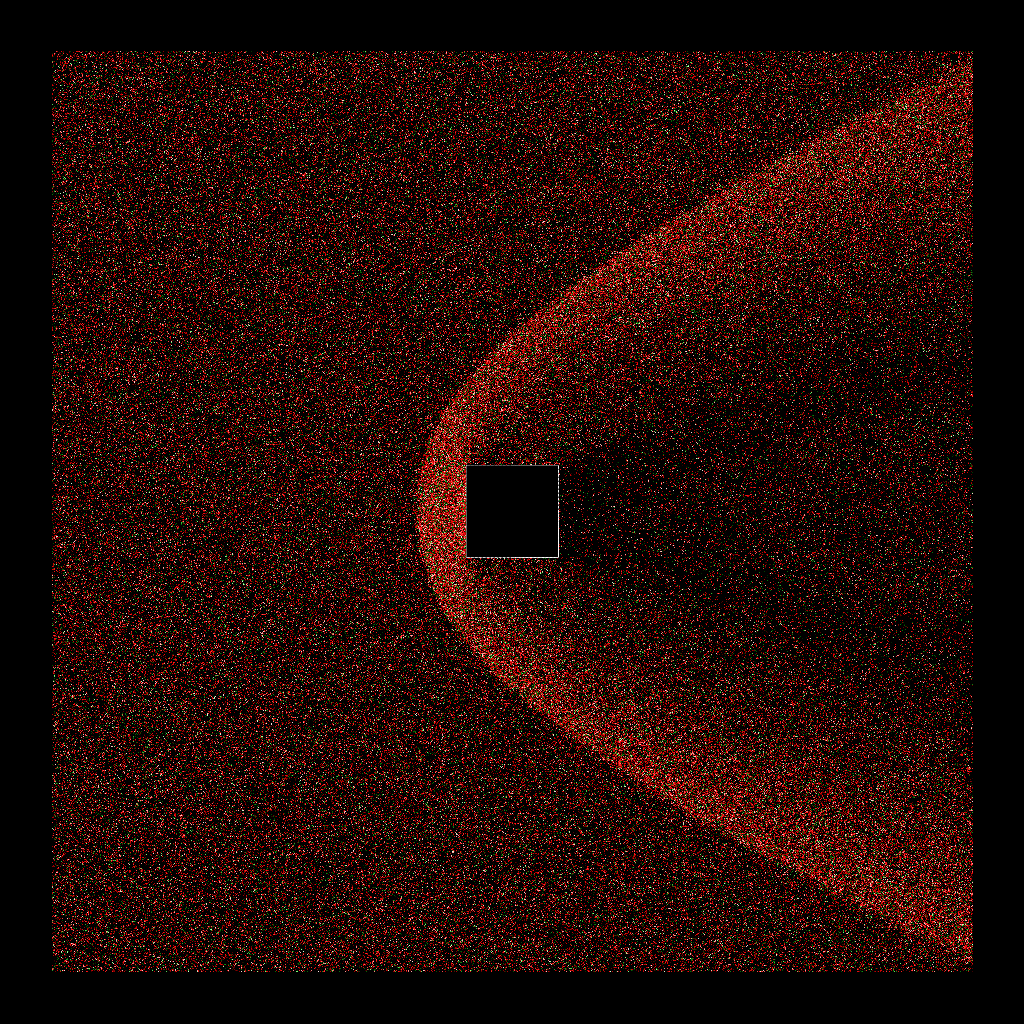
\includegraphics[width=\textwidth]{Images/4. Results/Square Kn/particles/Kn0.01.png}
        \caption{Kn = 0.01}
    \end{subfigure}
    \hfill
    \begin{subfigure}{0.32\textwidth}
        \centering
        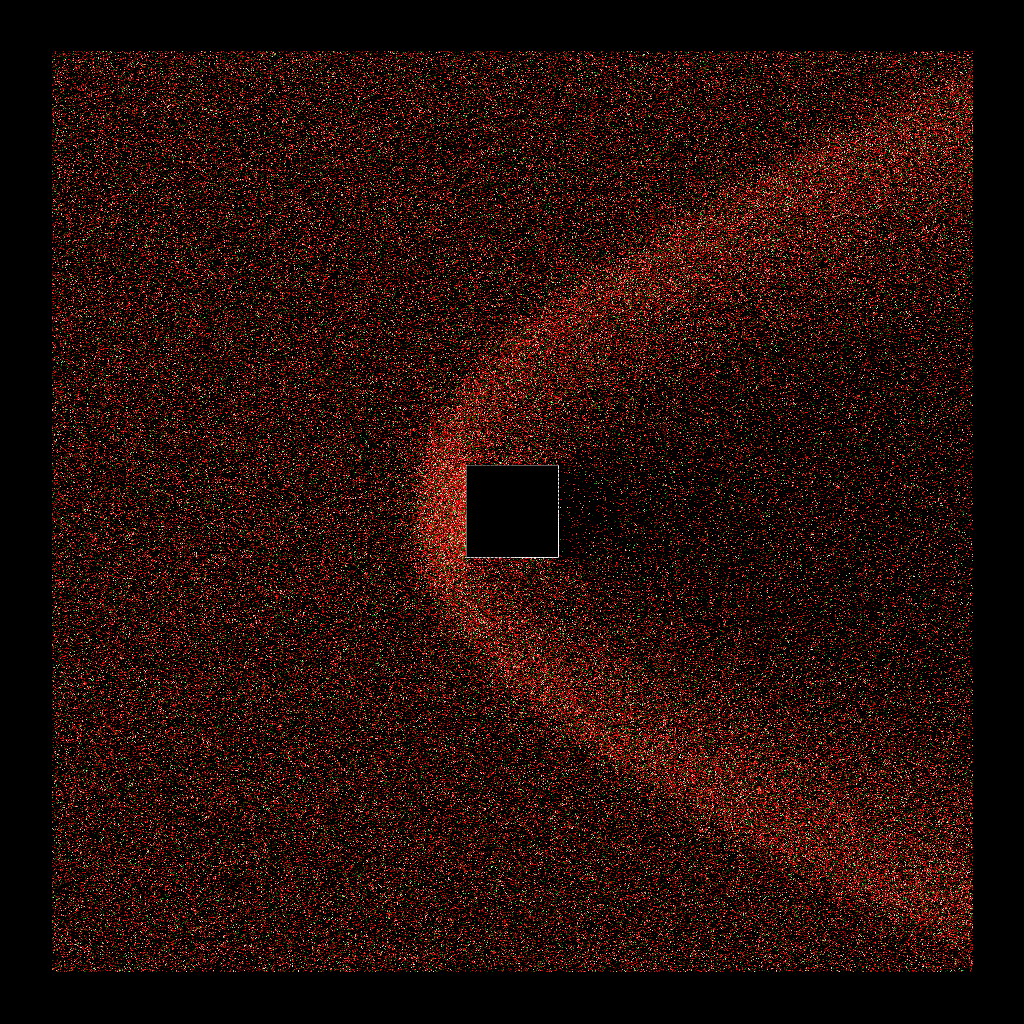
\includegraphics[width=\textwidth]{Images/4. Results/Square Kn/particles/Kn0.05.png}
        \caption{Kn = 0.05}
    \end{subfigure}
    
    \vspace{5pt}
    
    \centering
    \begin{subfigure}{0.32\textwidth}
        \centering
        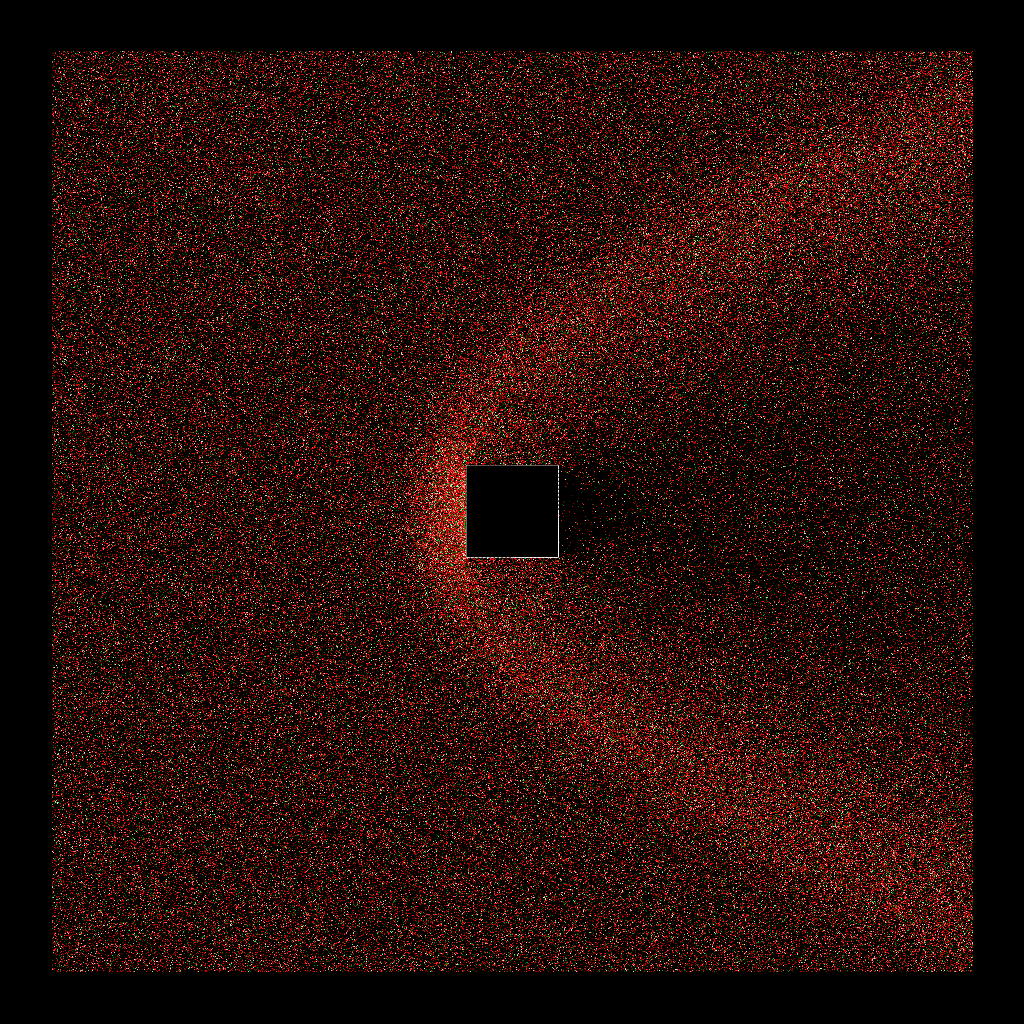
\includegraphics[width=\textwidth]{Images/4. Results/Square Kn/particles/Kn0.1.png}
        \caption{Kn = 0.1}
    \end{subfigure}
    \hfill
    \begin{subfigure}{0.32\textwidth}
        \centering
        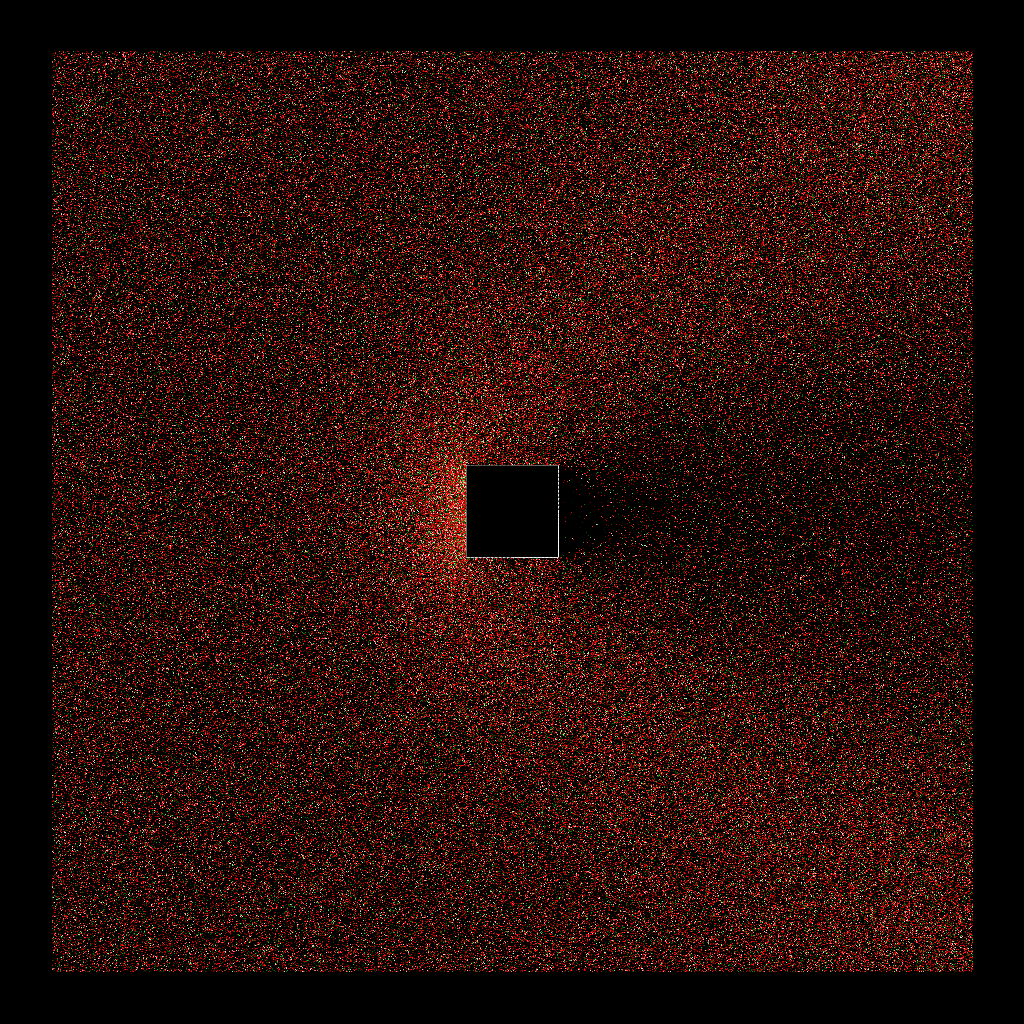
\includegraphics[width=\textwidth]{Images/4. Results/Square Kn/particles/Kn0.5.png}
        \caption{Kn = 0.5}
    \end{subfigure}
    \hfill
    \begin{subfigure}{0.32\textwidth}
        \centering
        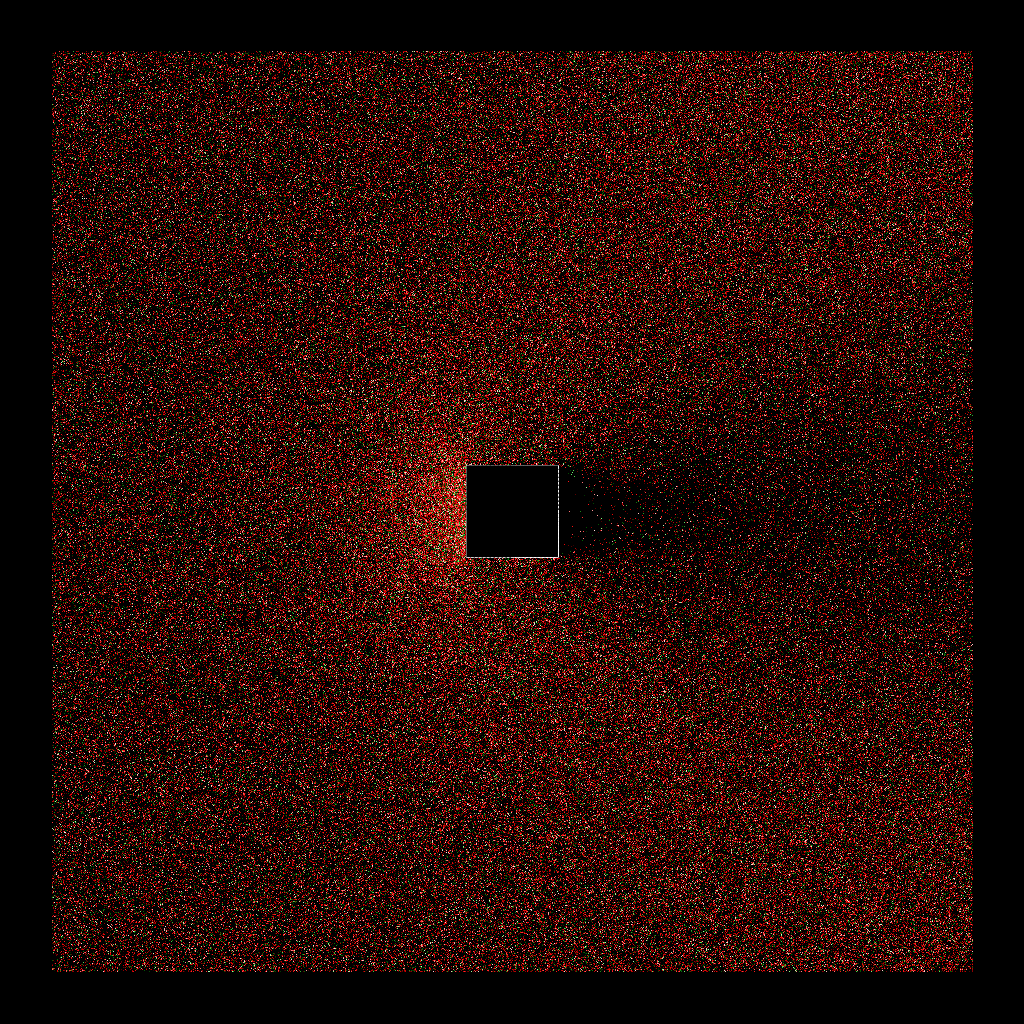
\includegraphics[width=\textwidth]{Images/4. Results/Square Kn/particles/Kn1.png}
        \caption{Kn = 1}
    \end{subfigure}
    
    \vspace{5pt}
    
    \centering
    \begin{subfigure}{0.32\textwidth}
        \centering
        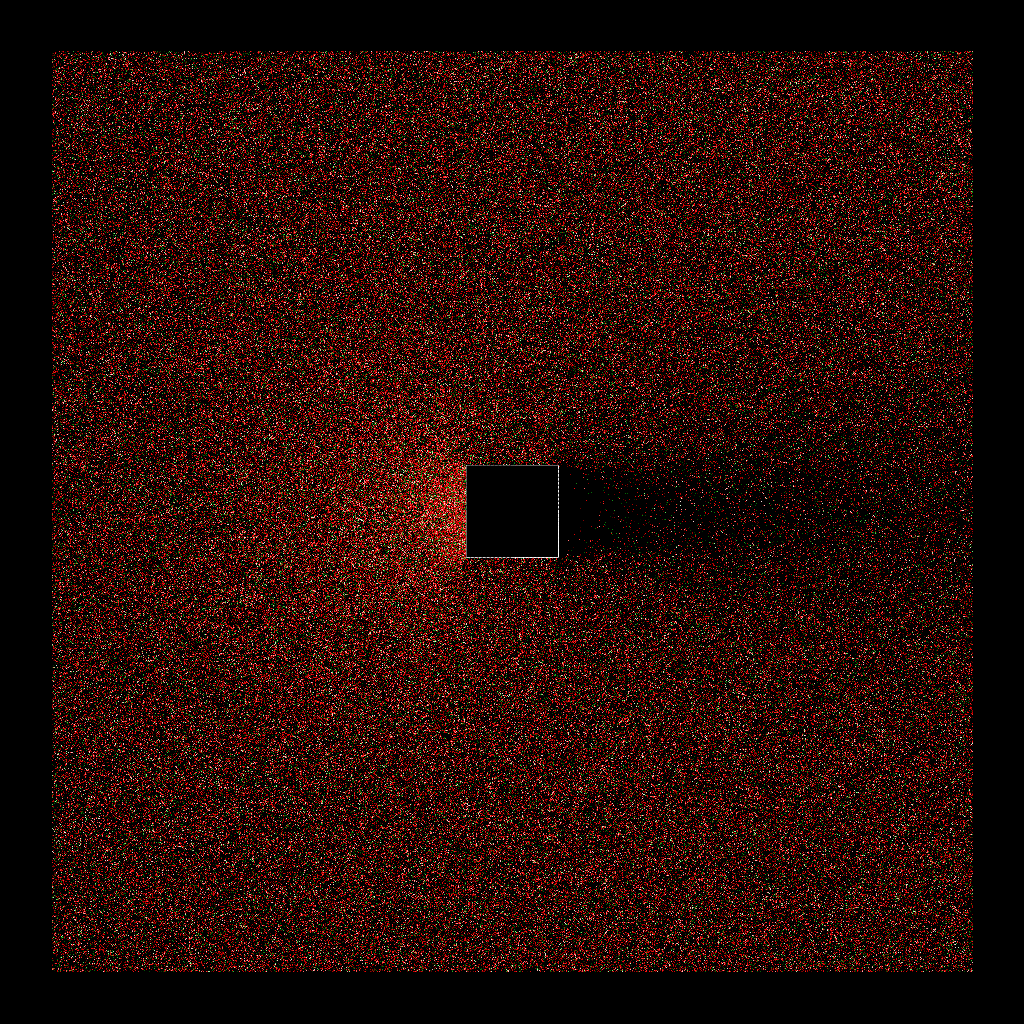
\includegraphics[width=\textwidth]{Images/4. Results/Square Kn/particles/Kn5.png}
        \caption{Kn = 5}
    \end{subfigure}
    \hfill
    \begin{subfigure}{0.32\textwidth}
        \centering
        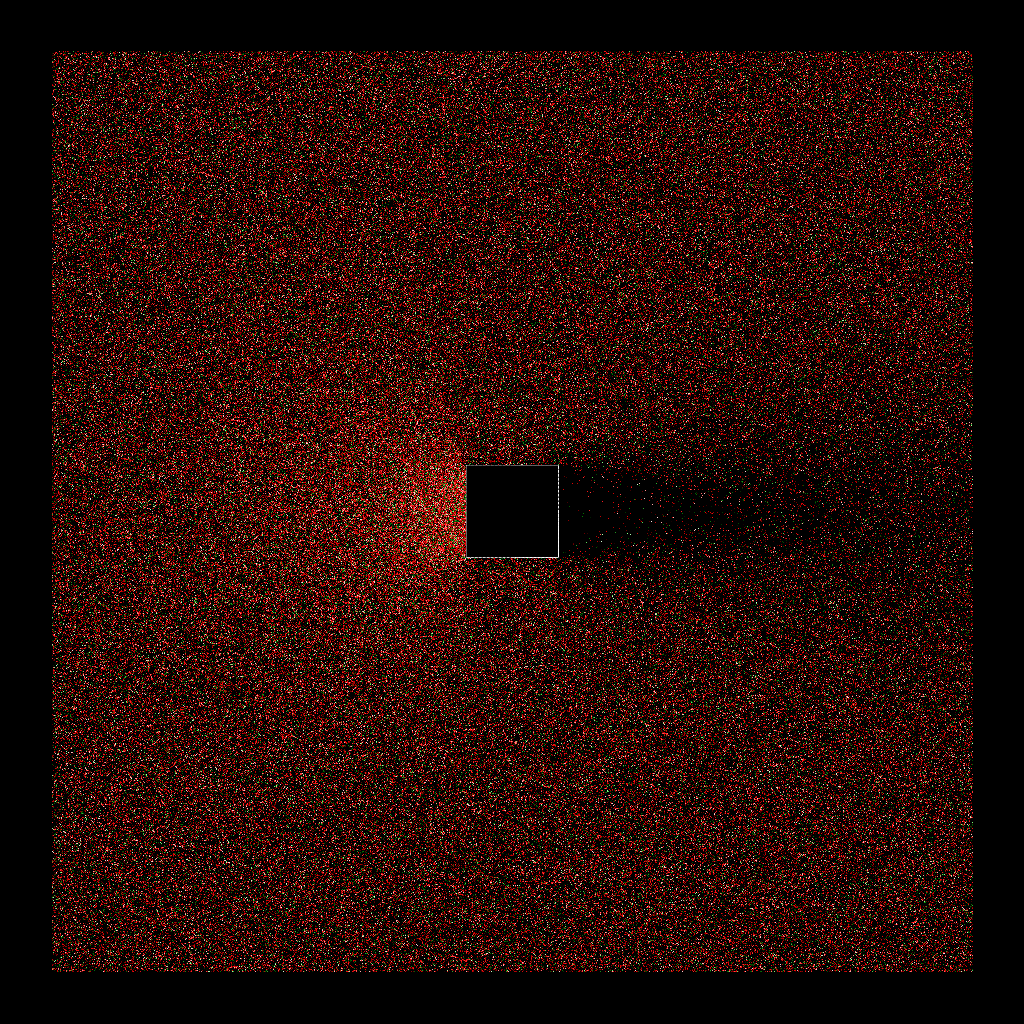
\includegraphics[width=\textwidth]{Images/4. Results/Square Kn/particles/Kn10.png}
        \caption{Kn = 10}
    \end{subfigure}
    \hfill
    \begin{subfigure}{0.32\textwidth}
        \centering
        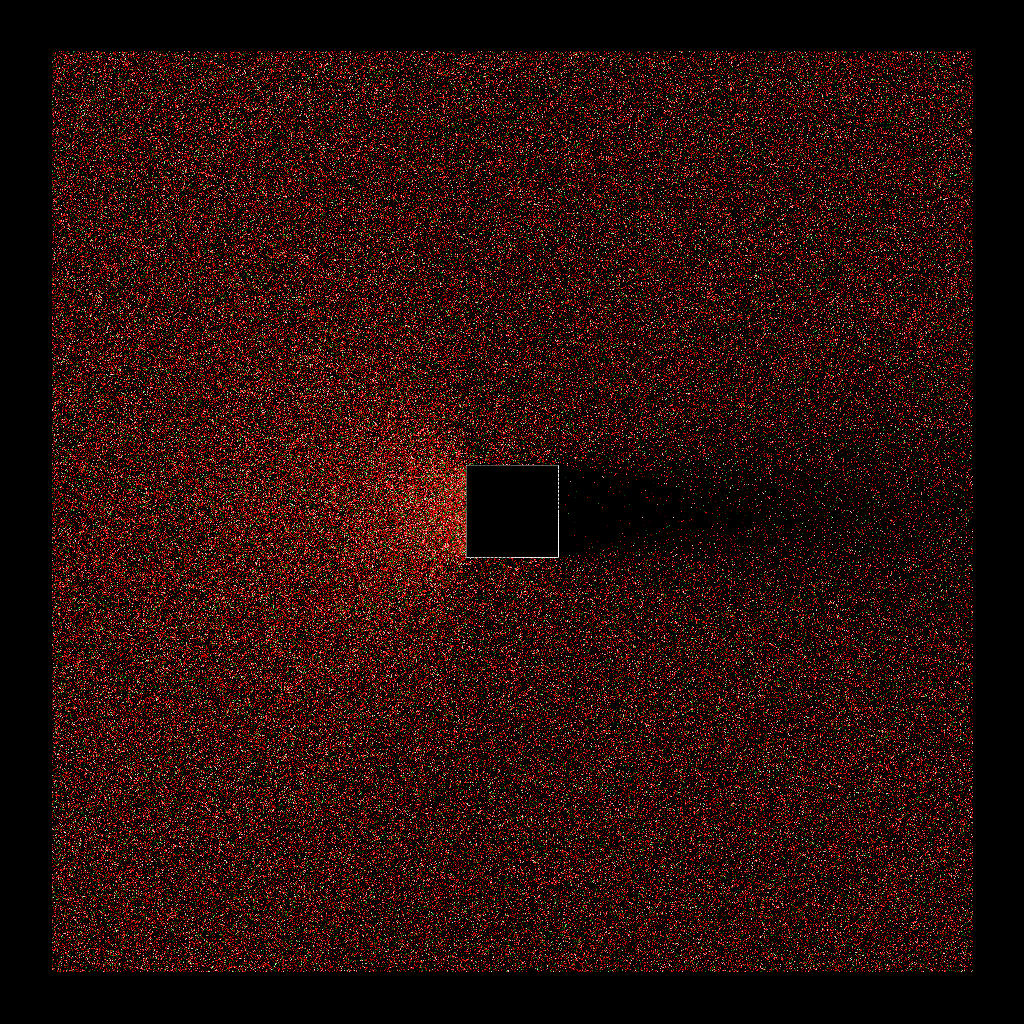
\includegraphics[width=\textwidth]{Images/4. Results/Square Kn/particles/Kn100.png}
        \caption{Kn = 100}
    \end{subfigure}
    \caption{Particle contours around a rounded square for varying Knudsen number.}
    \label{fig:pcontoursquare}
\end{figure}

\begin{figure}
    \centering
    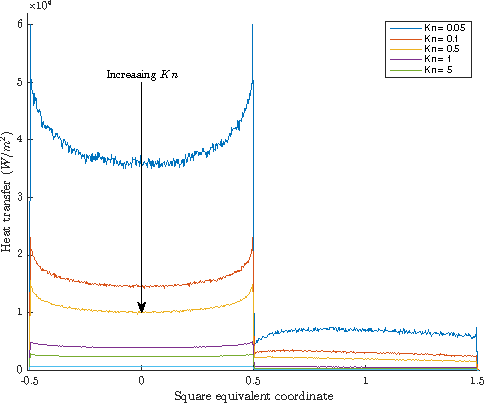
\includegraphics[width=0.52\textwidth]{Images/4. Results/Square Kn/htsec.pdf}
    \caption{Distribution of heat transfer along the square contour for varying values of Knudsen number}
    \label{fig:squarehtsec}
\end{figure}

\begin{figure}
    \centering
    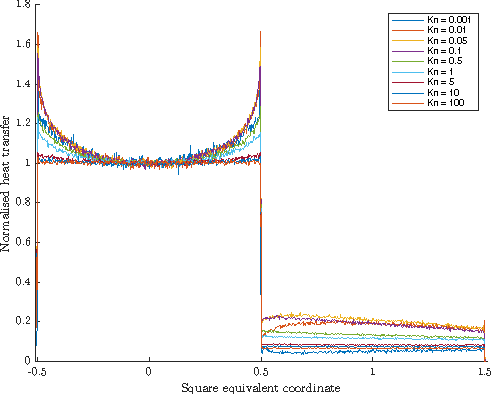
\includegraphics[width=0.52\textwidth]{Images/4. Results/Square Kn/nhtsec.pdf}
    \caption{Distribution of normalised heat transfer along the square contour for varying values of Knudsen number}
    \label{fig:squarenhtsec}
\end{figure}

\begin{figure}
    \centering
    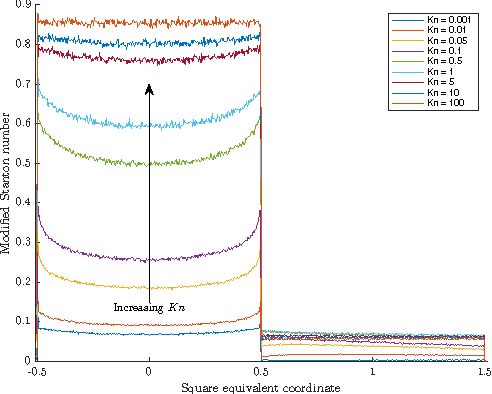
\includegraphics[width=0.52\textwidth]{Images/4. Results/Square Kn/stsec.pdf}
    \caption{Distribution of modified Stanton number along the square contour for varying values of Knudsen number}
    \label{fig:squarestsec}
\end{figure}

\autoref{fig:squarehtsec} shows the distribution of heat transfer along the square contour for varying values of Knudsen number. A very significant reduction in heat transfer is observed with increased Knudsen number. This is probably caused by the decrease in density of the flow.

\autoref{fig:squarenhtsec} shows the heat transfer contours normalised by stagnation point heating. Peaks in heat transfer similar to those noted in \cite{rees} can be seen at the corners of the square for low Knudsen numbers. These peaks, however, disappear as the Knudsen number is increased. This is probably due to the change in flow physics explained above: as the flow is not forced to turn around the corner, its velocity does not increase and as a result the heat transfer profile flattens out.

\autoref{fig:squarestsec} shows the distribution of modified Stanton number along the square contour for varying of Knudsen numbers. The significant increase in Stanton number seen with increasing Knudsen number can again be probably explained by the change in flow physics with Knudsen number: as $Kn$ is increased, the high density region between the shock and the cube's stagnation surface gradually dissipates, disappearing completely at very high Knudsen numbers. Consequently, the particles that collide with the cube's surface lose less energy, as they don't undergo collisions with molecules in the high-density region. This results in an higher energy transfer during the subsequent impact with the cube, leading to an increase in Stanton number.


Similar flow physics and heating trends were observed for a circle geometry. They can be seen in \autoref{fig:vcontourcircle} and \autoref{fig:heatcontourcircle}. 

\begin{figure}
    \centering
    \begin{subfigure}{0.32\textwidth}
        \centering
        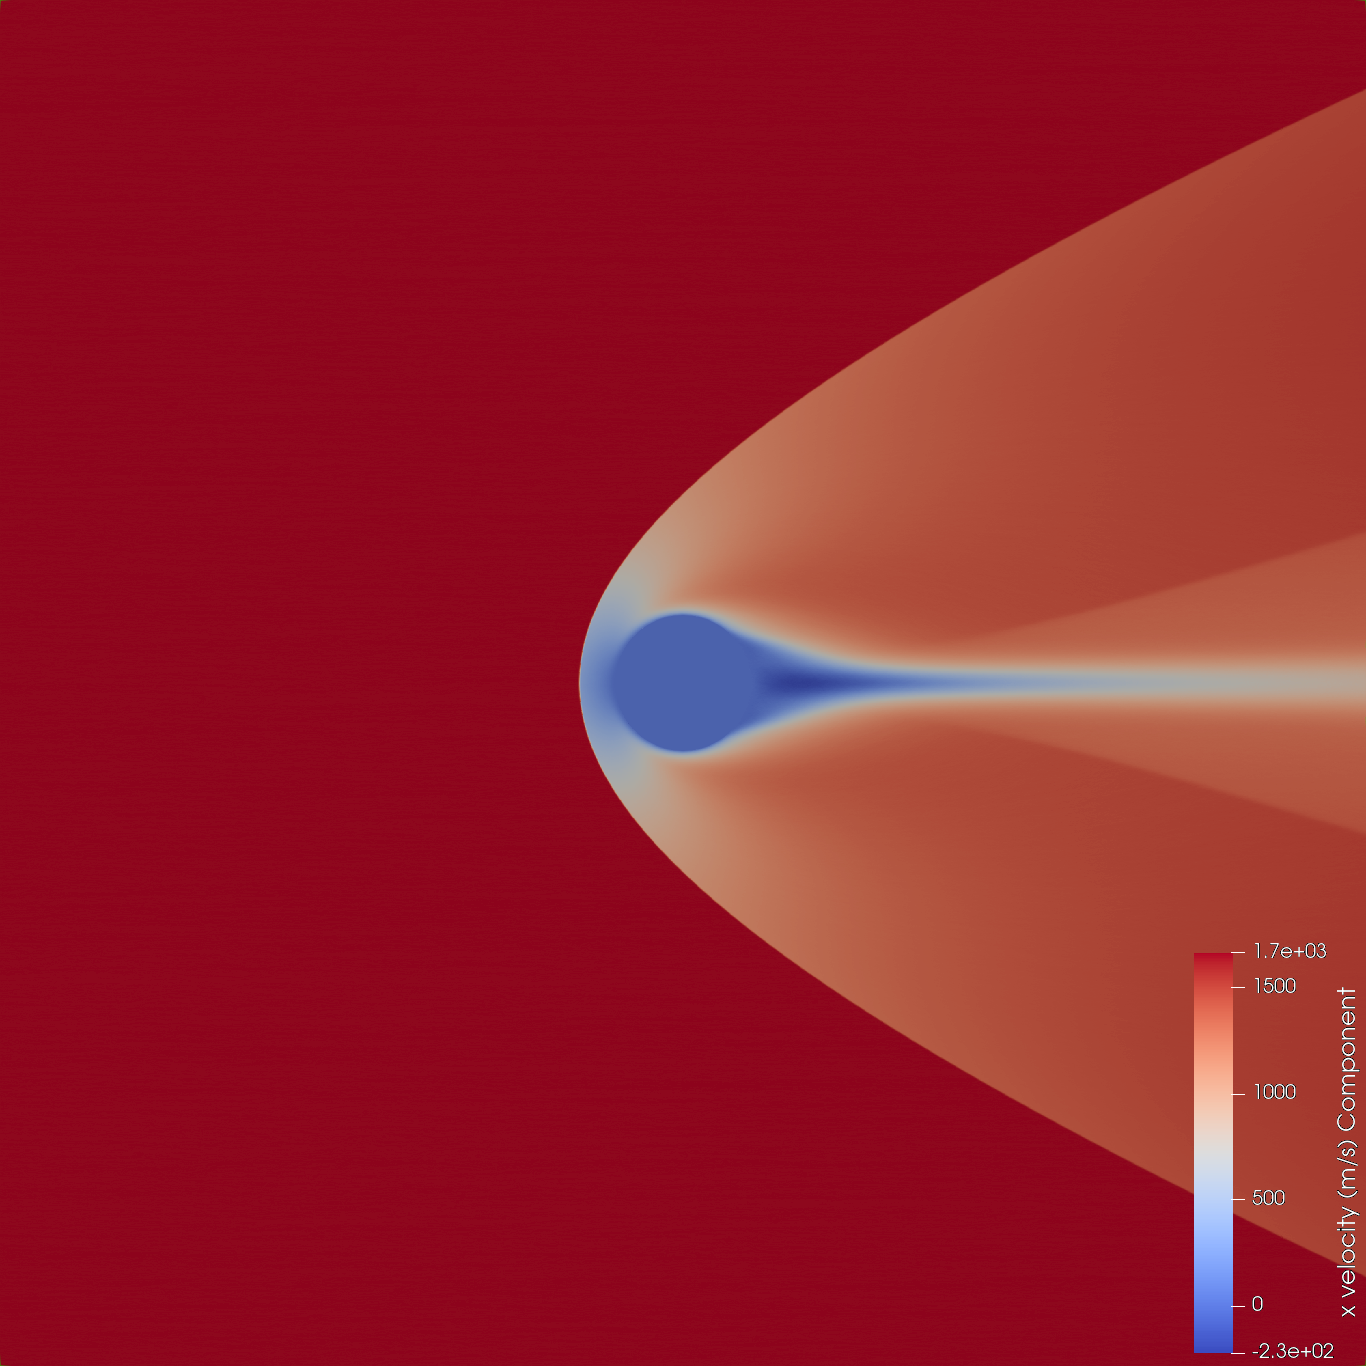
\includegraphics[width=\textwidth]{Images/4. Results/Circle Kn/pv/Kn0.001.png}
        \caption{Kn = 0.001}
    \end{subfigure}
    \hfill
    \begin{subfigure}{0.32\textwidth}
        \centering
        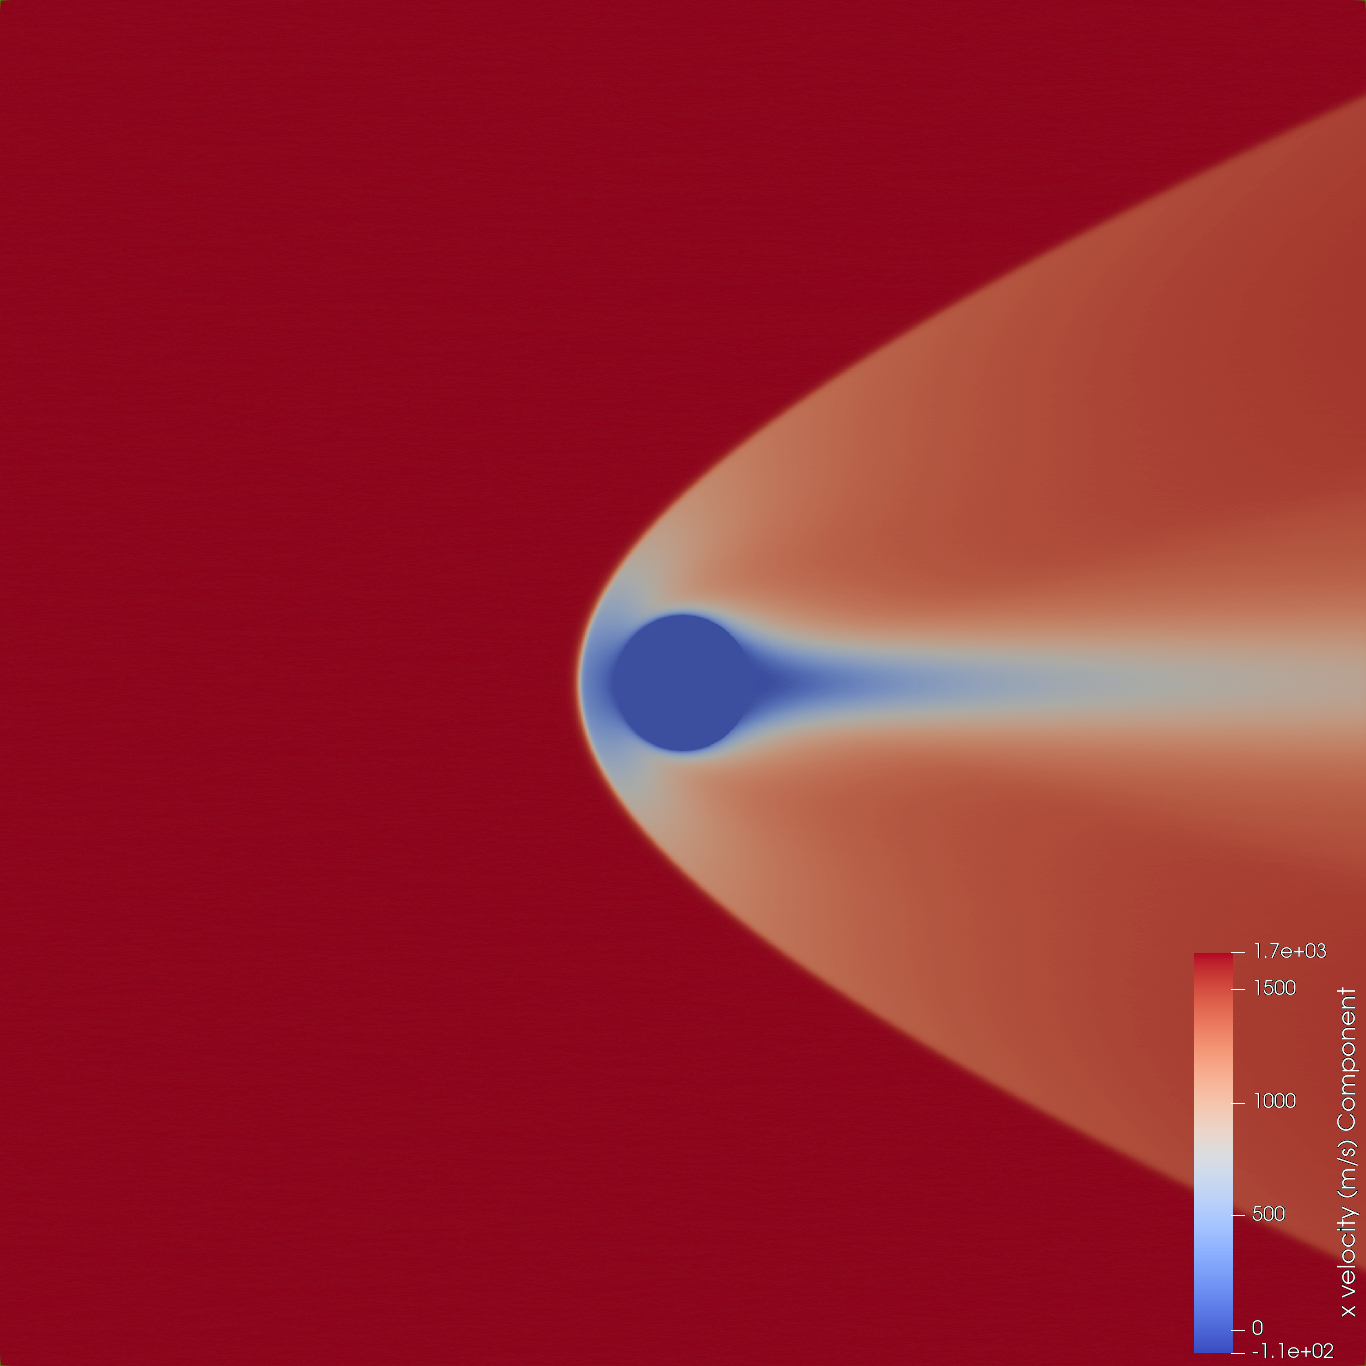
\includegraphics[width=\textwidth]{Images/4. Results/Circle Kn/pv/Kn0.01.png}
        \caption{Kn = 0.01}
    \end{subfigure}
    \hfill
    \begin{subfigure}{0.32\textwidth}
        \centering
        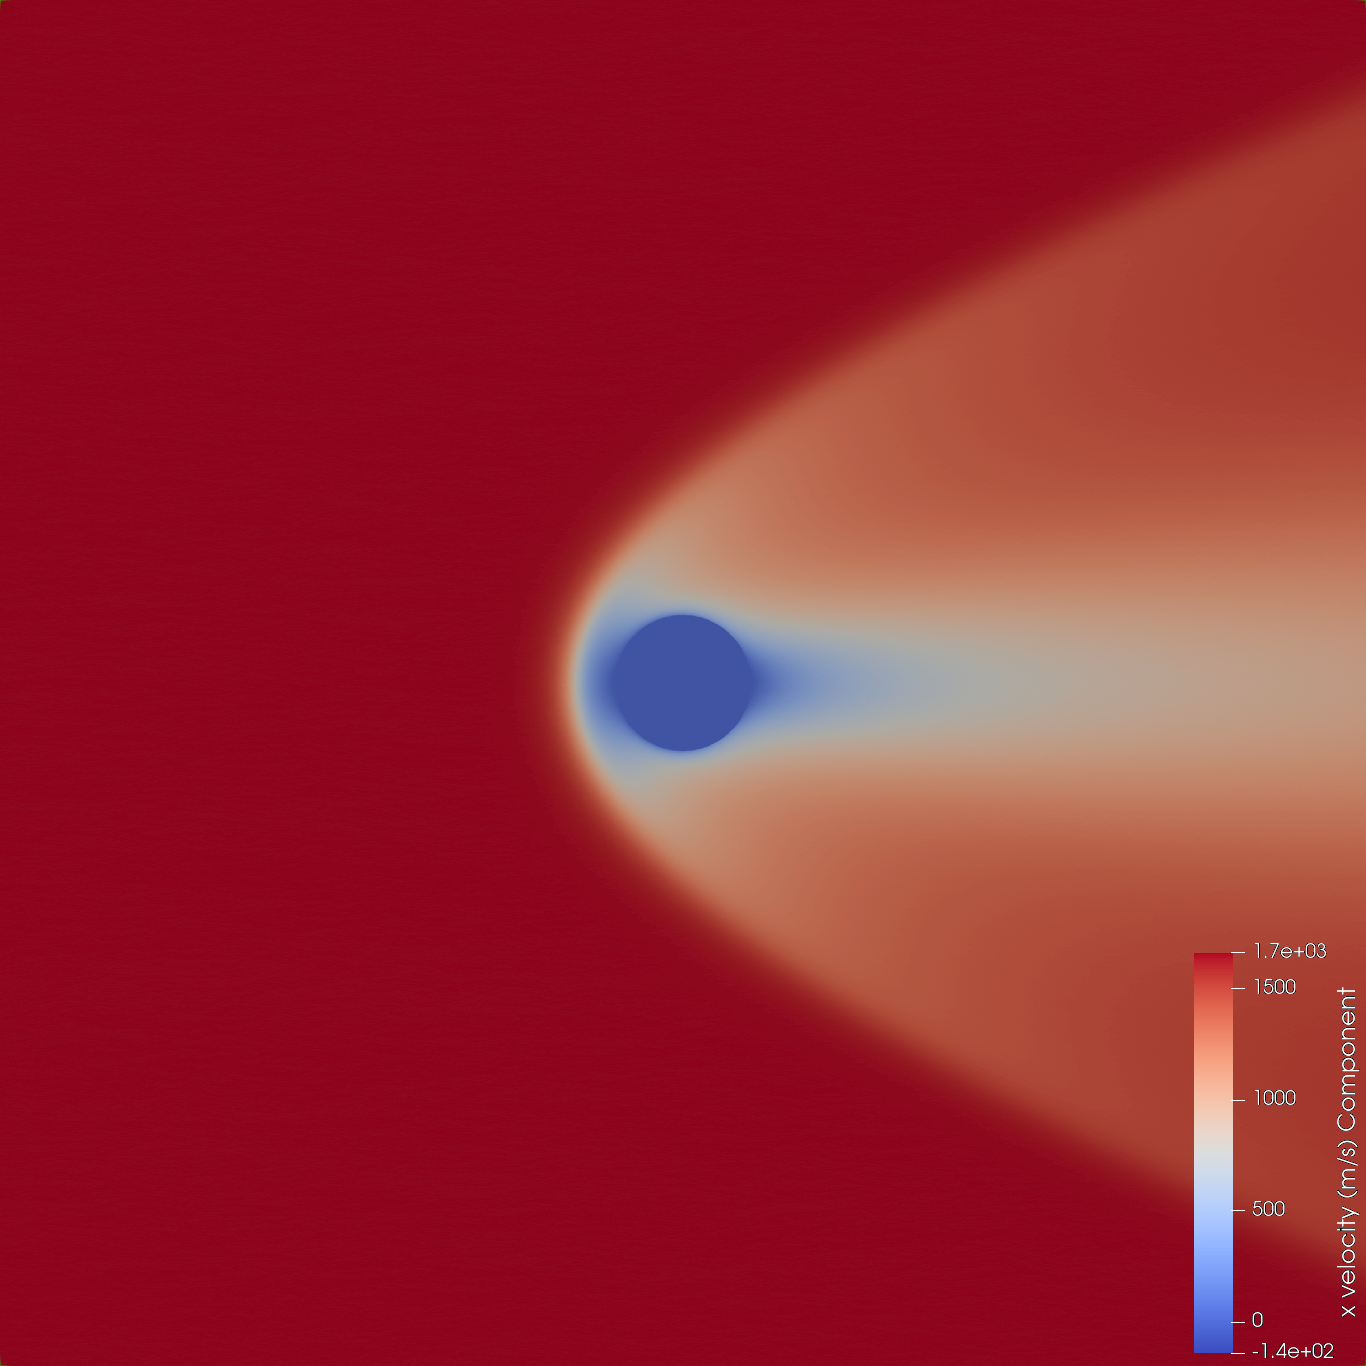
\includegraphics[width=\textwidth]{Images/4. Results/Circle Kn/pv/Kn0.05.png}
        \caption{Kn = 0.05}
    \end{subfigure}
    
    \vspace{5pt}
    
    \centering
    \begin{subfigure}{0.32\textwidth}
        \centering
        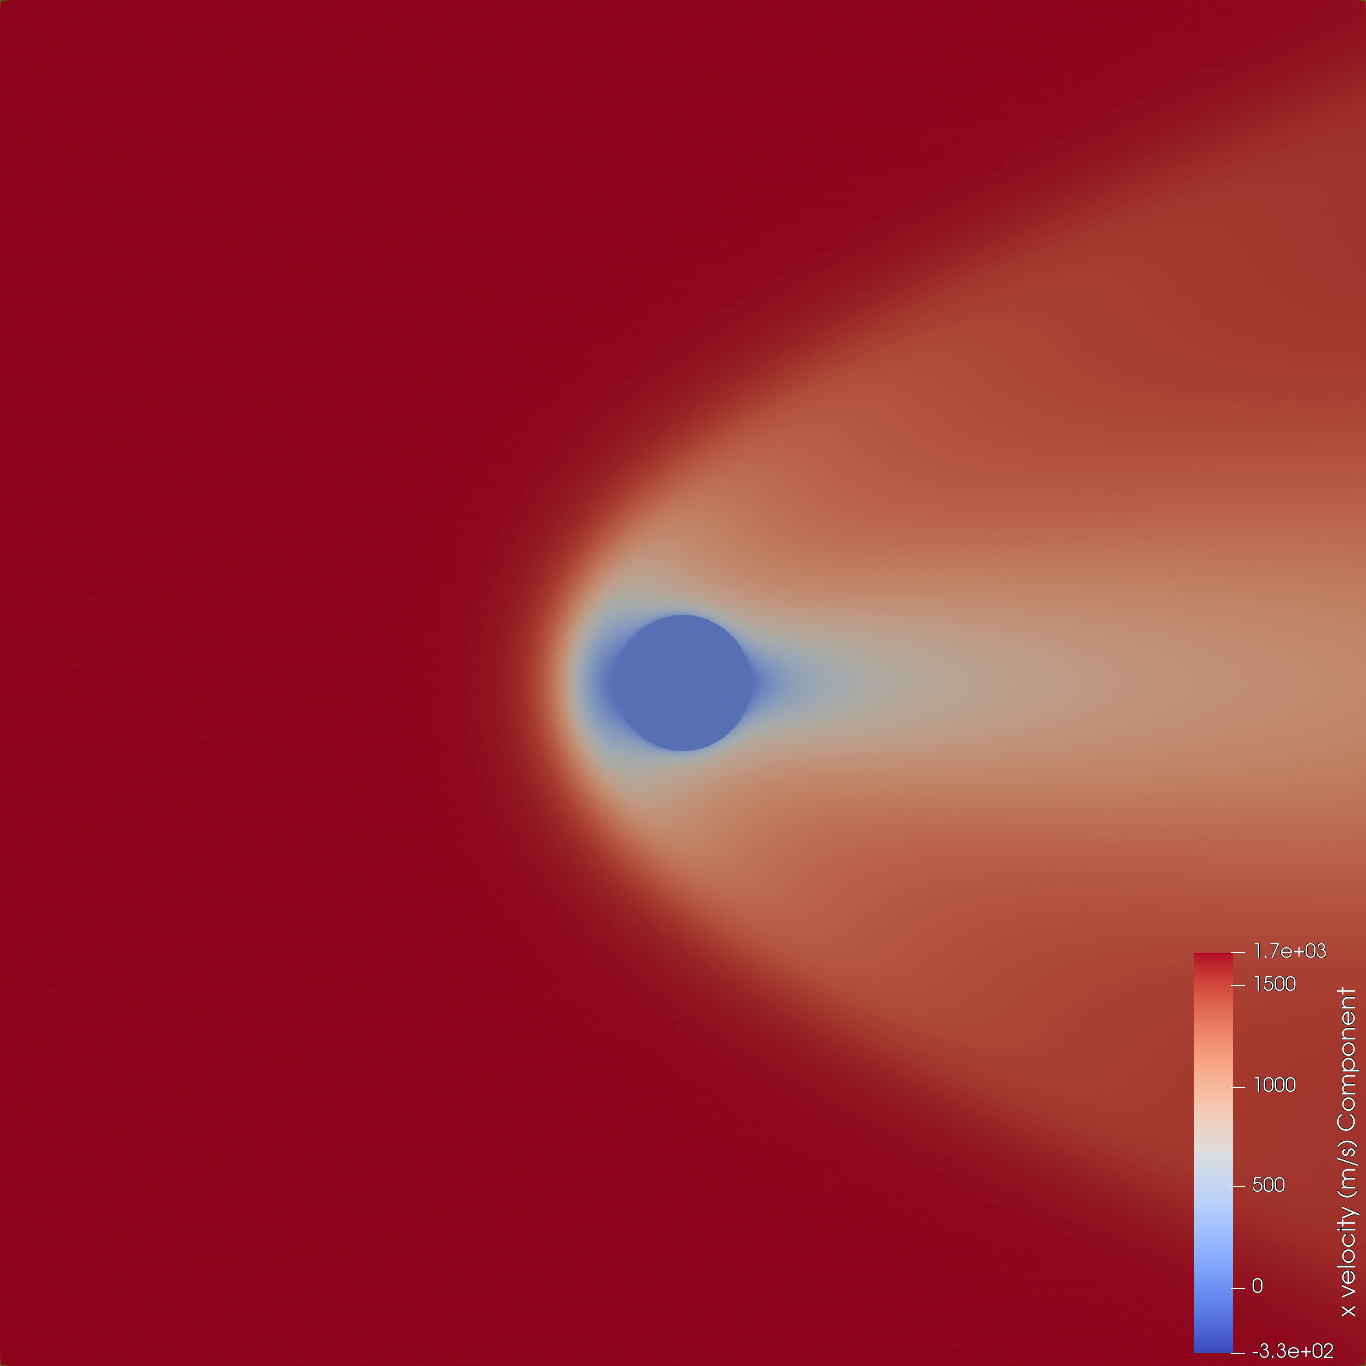
\includegraphics[width=\textwidth]{Images/4. Results/Circle Kn/pv/Kn0.1.png}
        \caption{Kn = 0.1}
    \end{subfigure}
    \hfill
    \begin{subfigure}{0.32\textwidth}
        \centering
        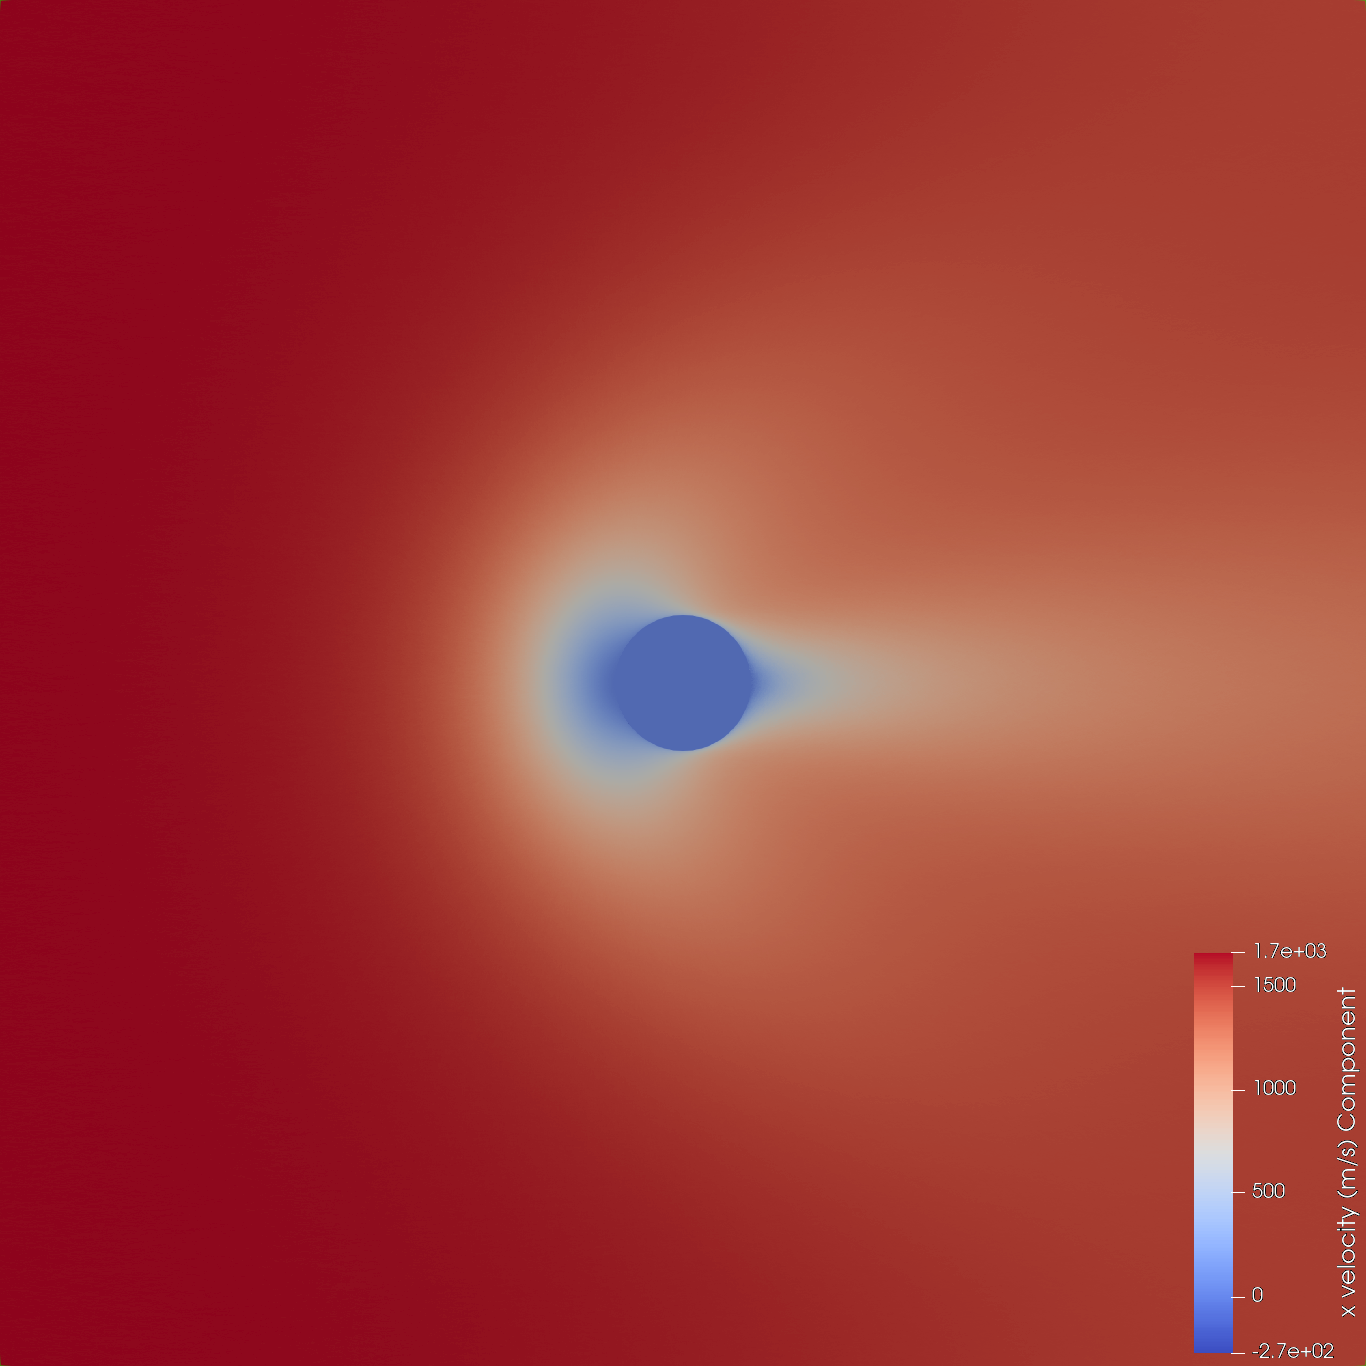
\includegraphics[width=\textwidth]{Images/4. Results/Circle Kn/pv/Kn0.5.png}
        \caption{Kn = 0.5}
    \end{subfigure}
    \hfill
    \begin{subfigure}{0.32\textwidth}
        \centering
        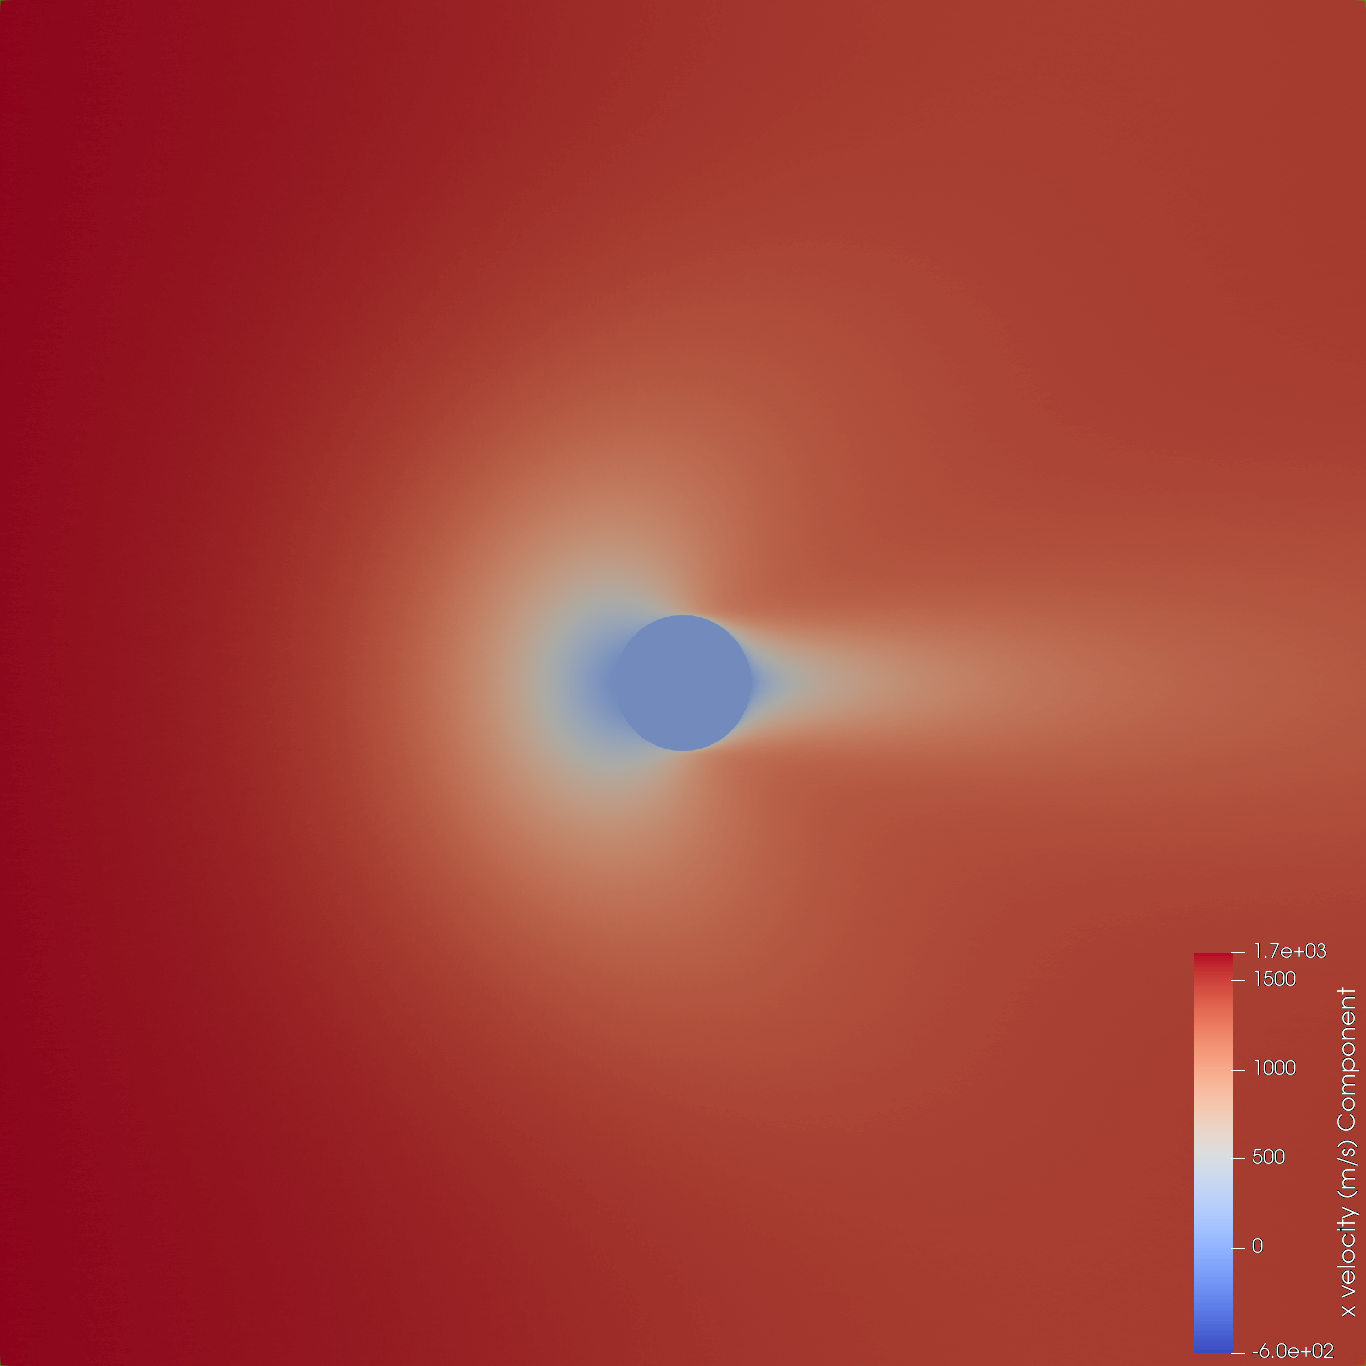
\includegraphics[width=\textwidth]{Images/4. Results/Circle Kn/pv/Kn1.png}
        \caption{Kn = 1}
    \end{subfigure}
    
    \vspace{5pt}
    
    \centering
    \begin{subfigure}{0.32\textwidth}
        \centering
        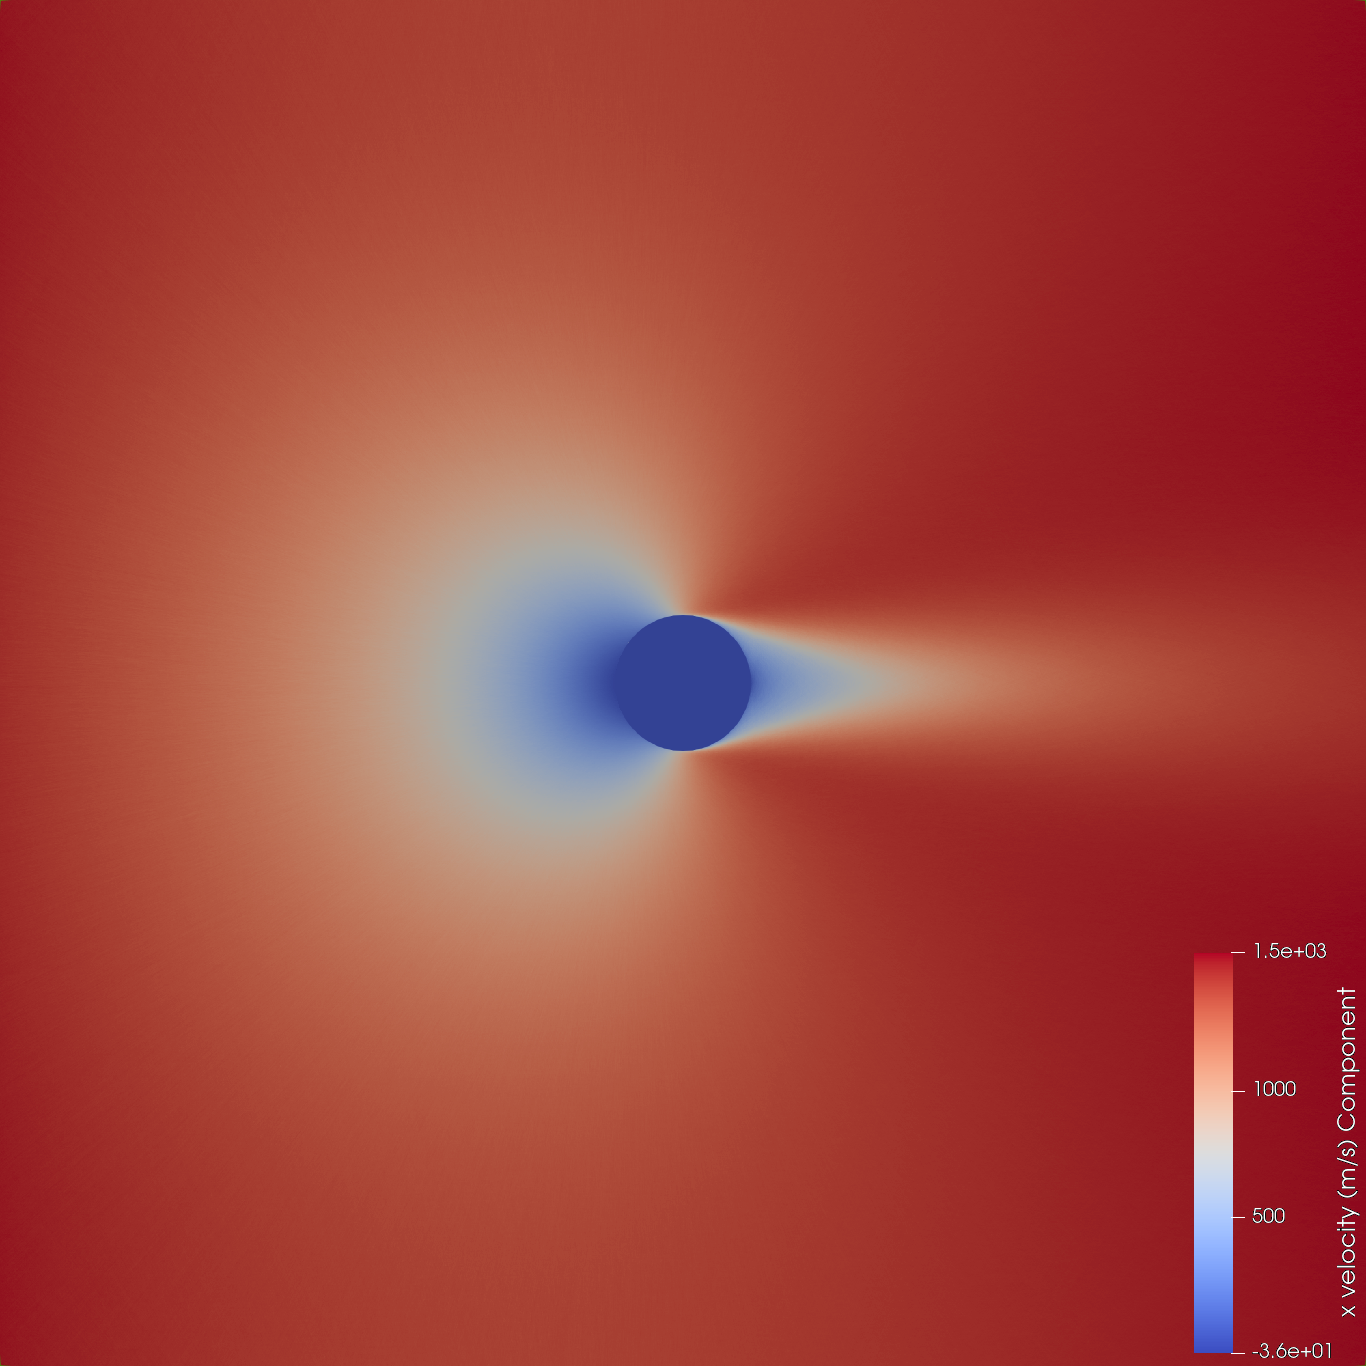
\includegraphics[width=\textwidth]{Images/4. Results/Circle Kn/pv/Kn5.png}
        \caption{Kn = 5}
    \end{subfigure}
    \hfill
    \begin{subfigure}{0.32\textwidth}
        \centering
        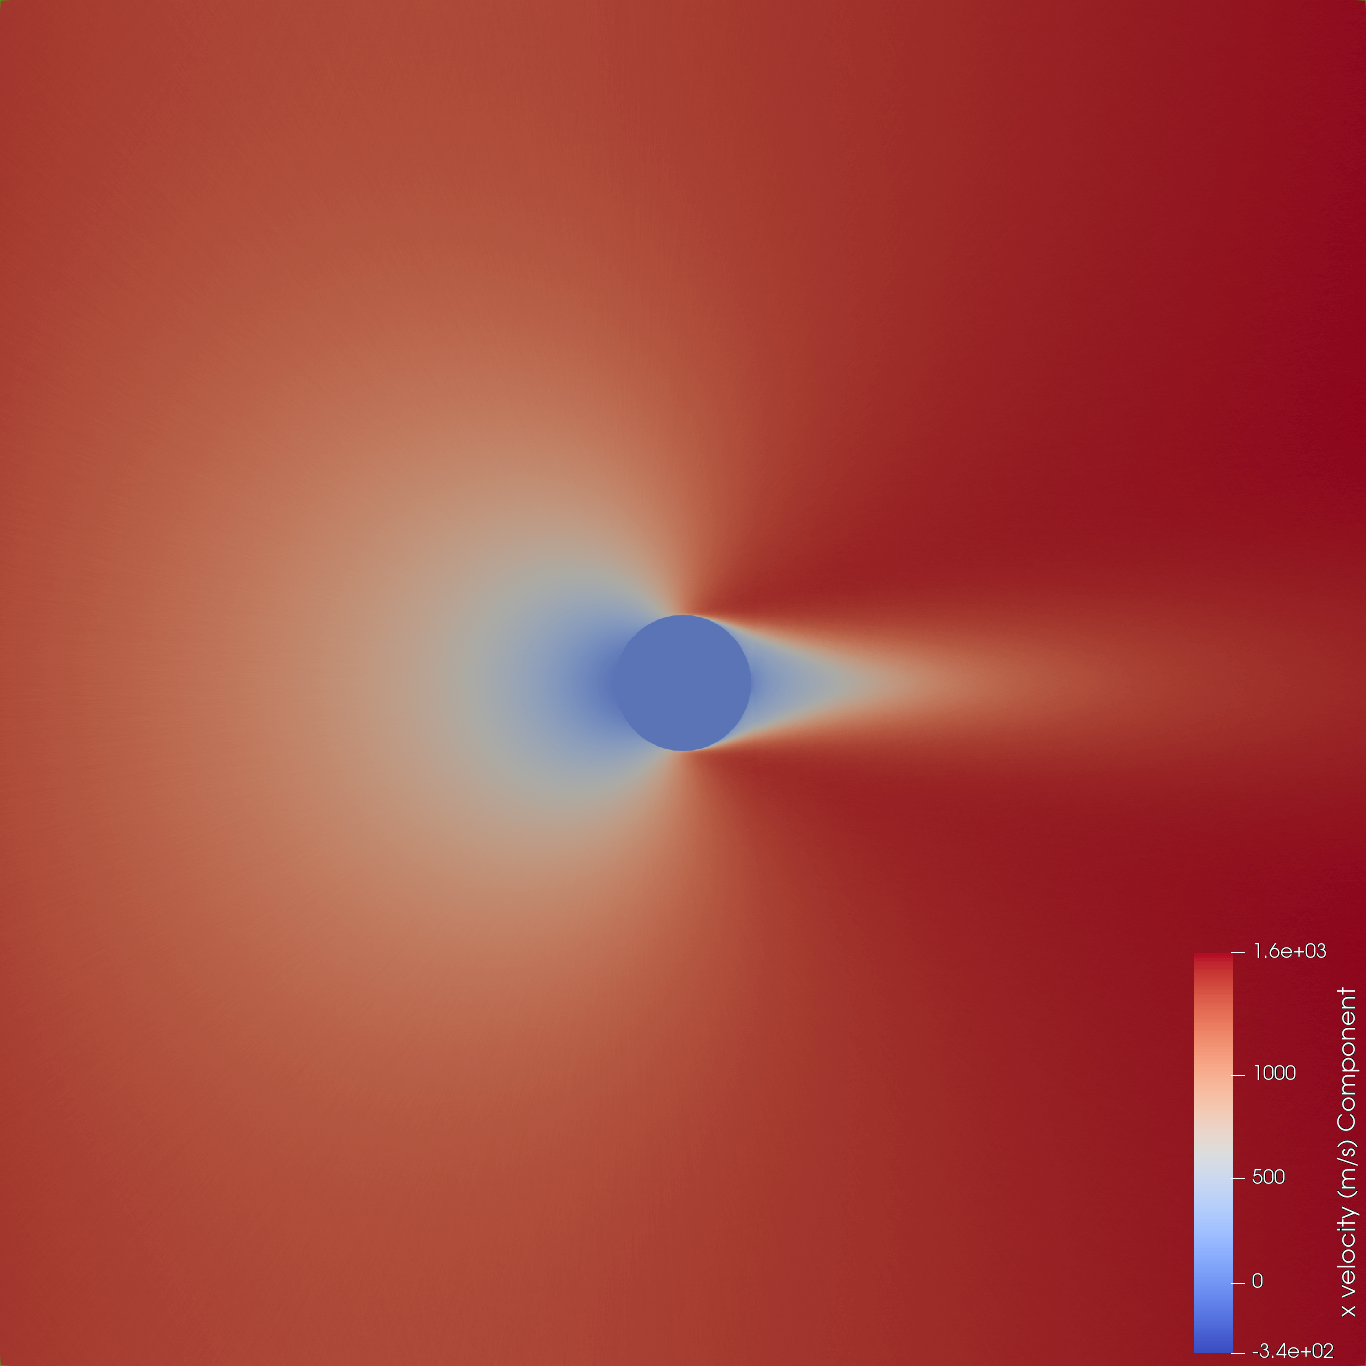
\includegraphics[width=\textwidth]{Images/4. Results/Circle Kn/pv/Kn10.png}
        \caption{Kn = 10}
    \end{subfigure}
    \hfill
    \begin{subfigure}{0.32\textwidth}
        \centering
        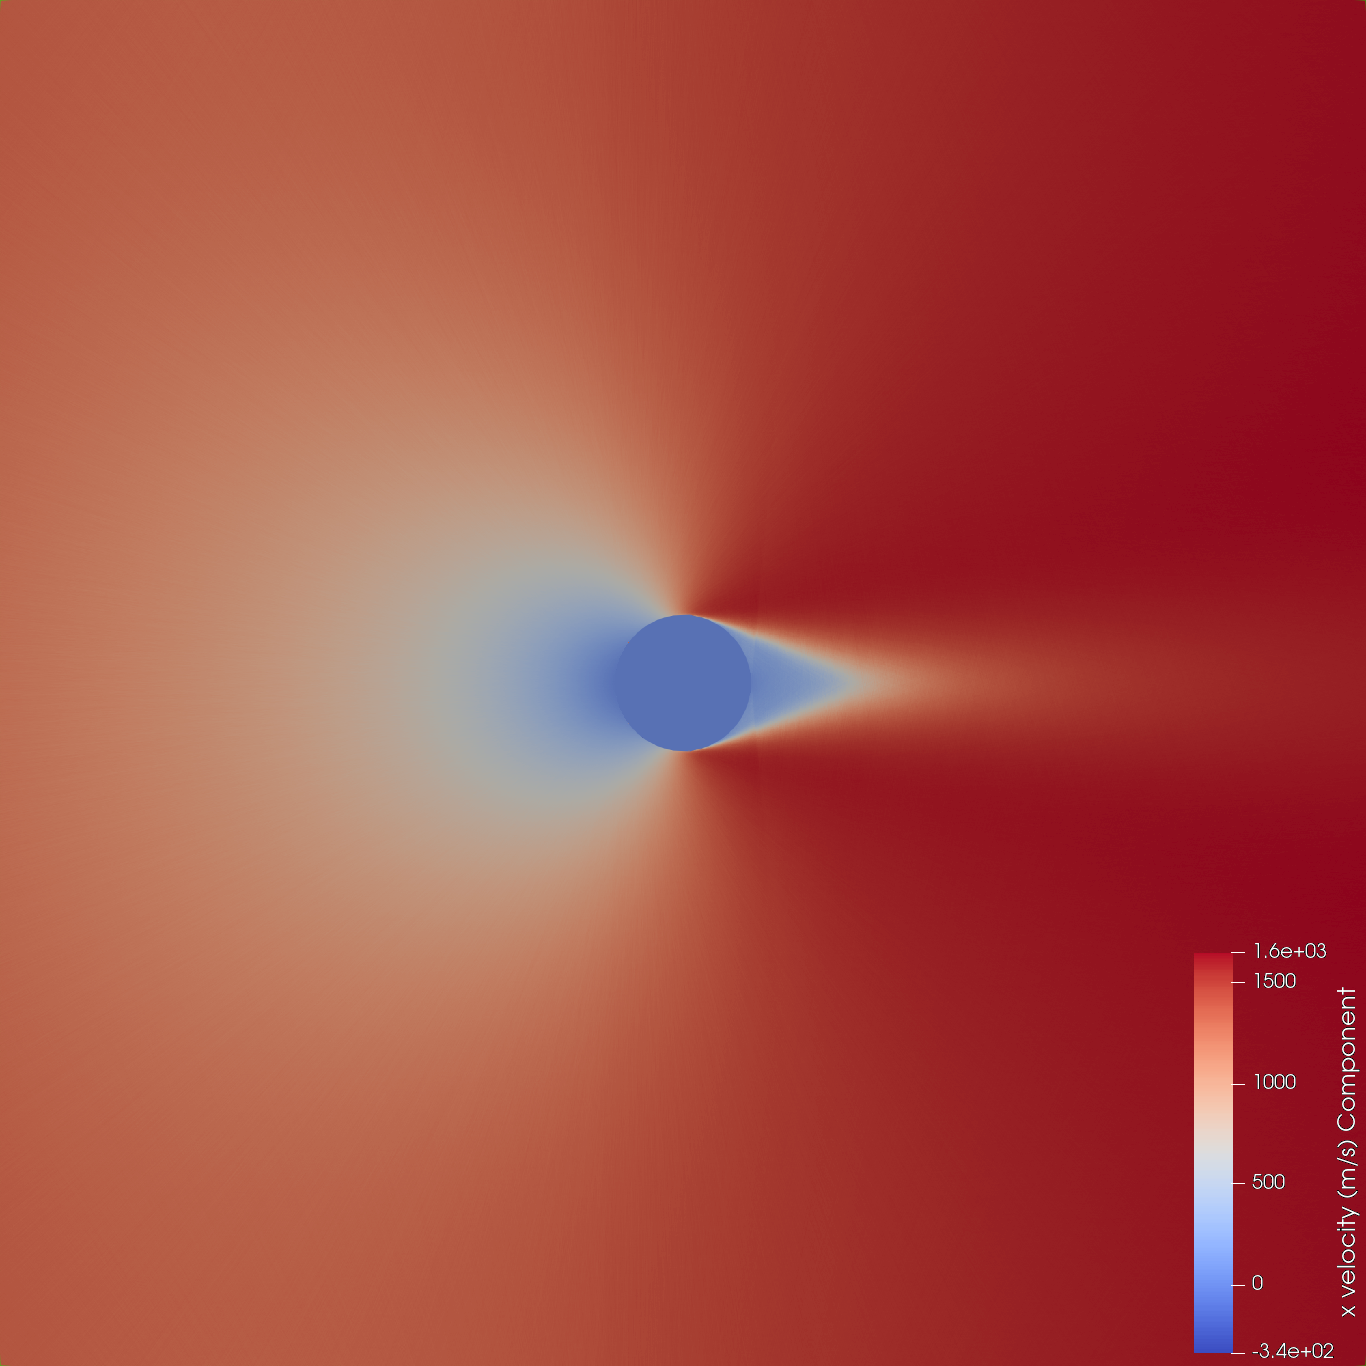
\includegraphics[width=\textwidth]{Images/4. Results/Circle Kn/pv/Kn100.png}
        \caption{Kn = 100}
    \end{subfigure}
    \caption{Velocity contours around a circle for varying Knudsen number.}
    \label{fig:vcontourcircle}
\end{figure}

\begin{figure}
    \centering
    \begin{subfigure}{0.49\textwidth}
        \centering
        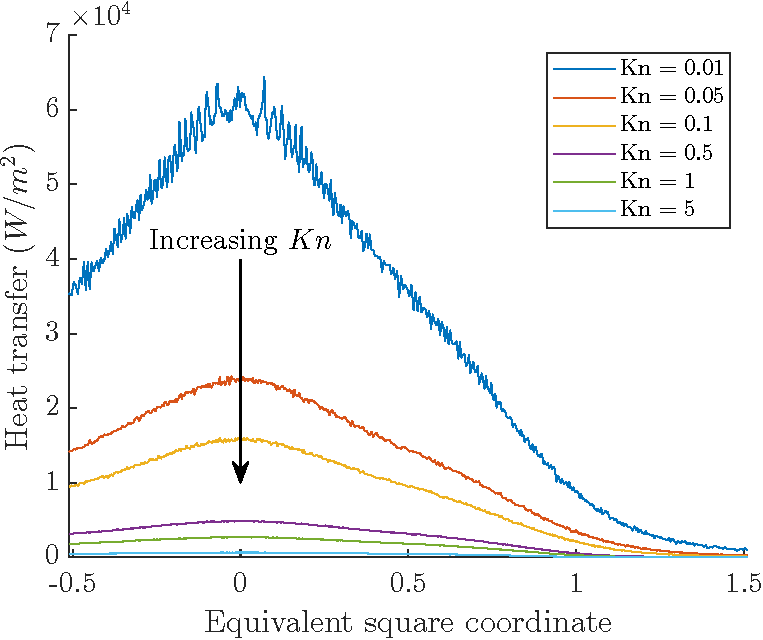
\includegraphics[width=\textwidth]{Images/4. Results/Circle Kn/htsec.pdf}
    \end{subfigure}
    \hfill
    \begin{subfigure}{0.49\textwidth}
        \centering
        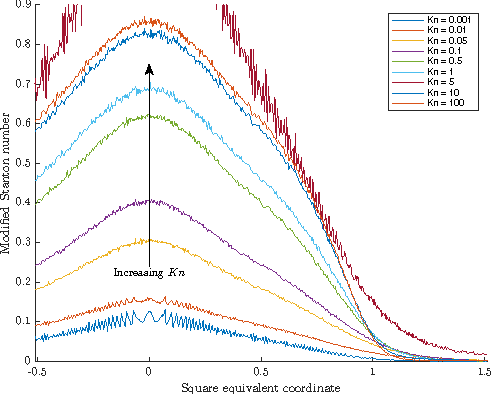
\includegraphics[width=\textwidth]{Images/4. Results/Circle Kn/stsec.pdf}
    \end{subfigure}
    \caption{Heating (left) and stagnation Stanton number (right) distribution around a circle for varying Knudsen number.}
    \label{fig:heatcontourcircle}
\end{figure}

The variation in stagnation point Stanton number observed in \autoref{fig:squarestsec} and \autoref{fig:heatcontourcircle} have been plotted respectively in \autoref{fig:stantonsquare} and \autoref{fig:stantoncircle}, with respect to the global Knudsen number, calculated based on the square side length. The observed pattern is partly matched by the one observed in literature for spheres \cite{riabov}, shown in \autoref{fig:riabov}. The behaviour for Knudsen numbers below 0.01 could not be compared, due to lack of experimental data.

\begin{figure}
    \centering
    \begin{subfigure}{0.49\textwidth}
        \centering
        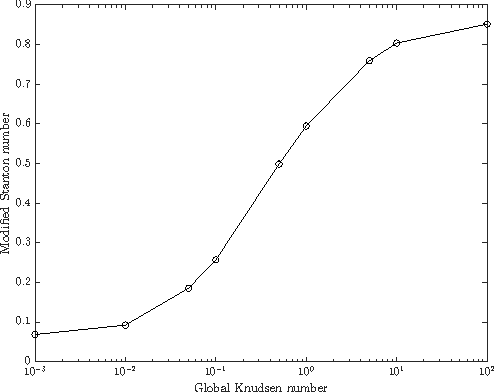
\includegraphics[width=\textwidth]{Images/4. Results/Square Kn/stkn.pdf}
        \caption{Square}
        \label{fig:stantonsquare}
    \end{subfigure}
    \hfill
    \begin{subfigure}{0.49\textwidth}
        \centering
        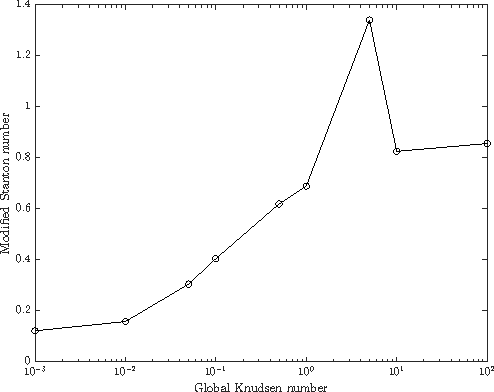
\includegraphics[width=\textwidth]{Images/4. Results/Circle Kn/stkn.pdf}
        \caption{Circle}
        \label{fig:stantoncircle}
    \end{subfigure}
    \caption{Stanton number vs global Knudsen number for a rounded square (a) and circle (b).}
    \label{fig:stanton}
\end{figure}

\begin{figure}
    \centering
    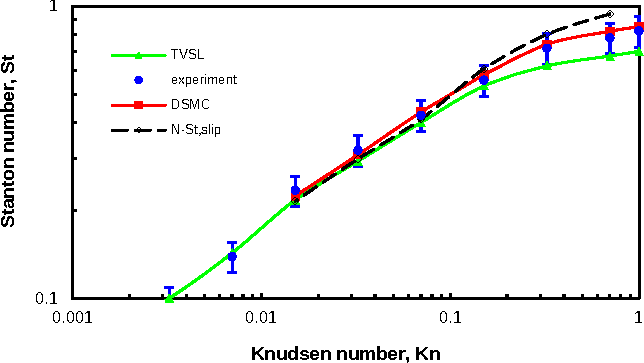
\includegraphics{Images/4. Results/riabov.pdf}
    \caption{Stanton number vs global Knudsen number from literature \cite{riabov}.}
    \label{fig:riabov}
\end{figure}

The variation in ratio between the peak and stagnation point Stanton number has been calculated and plotted against the local Knudsen number at the square corner. It can be seen in \autoref{fig:ratiokn}. The trend shown by it mostly appears as it would have been expected based on the intuition gained from the velocity contours above. The point at $Kn = 0.1$ is however, shows a slightly lower value from the peak at $Kn = 1$. The reason for this dip is not entirely clear, and will be discussed more in depth in \autoref{subsection:comparison}.

\begin{figure}
    \centering
    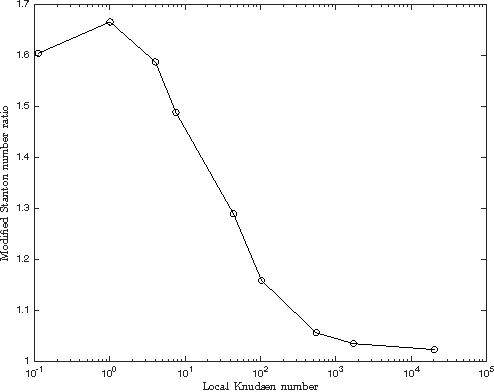
\includegraphics[width=0.6\textwidth]{Images/4. Results/Square Kn/stratiolocalkn.pdf}
    \caption{Stanton number ratio vs local Knudsen number for the varying global Knudsen number test case.}
    \label{fig:ratiokn}
\end{figure}

\subsection{Variation of edge radius results}

\autoref{fig:radiushtsec} shows the distribution of heat transfer around the geometry for varying values of edge radius. Note that, for clarity reasons, not all of the simulation cases have been included. It is possible to note that as the corner radius is increased, the reduction in heat transfer past the corner peak becomes more gradual, and the two peaks at the square edged coalesce into one. Because of the same effect, the heat transfer at the stagnation point gradually increases.

Comparing \autoref{fig:radiushtsec} to \autoref{fig:squarehtsec}, reveals that the order of magnitude reduction in heat transfer has disappeared, as the global Knudsen number (and thus the density) has been kept constant.

\begin{figure}
    \centering
    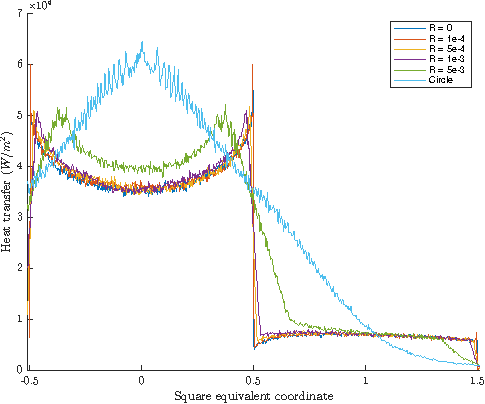
\includegraphics[width=0.52\textwidth]{Images/4. Results/Radius/htsec.pdf}
    \caption{Distribution of heat transfer along the square contour for varying values edge radius.}
    \label{fig:radiushtsec}
\end{figure}

\begin{figure}
    \centering
    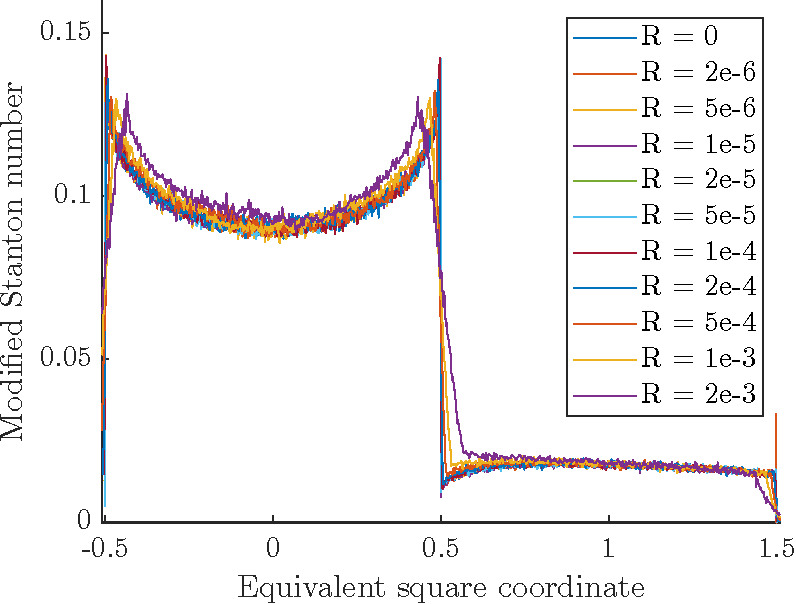
\includegraphics[width=0.52\textwidth]{Images/4. Results/Radius/stsec.pdf}
    \caption{Distribution of Stanton number along the square contour for varying values edge radius.}
    \label{fig:radiusstsec}
\end{figure}

\autoref{fig:radiusstsec} shows the Stanton number distribution around the geometry for varying values of edge radius (again, for clarity reasons only the test cases with comparatively small edge radius have been included). The distributions follows closely the one included in \autoref{fig:squarestsec} for $Kn = 0.01$, and very little change is observed for the peak Stanton number values (corresponding to the 0.5 point on the equivalent square coordinate axis) for varying values of edge radius. 



Plotting the Stanton number ratio against the local Knudsen number at the square corner (as shown in \autoref{fig:radiusstkn}) reveals an interesting trend. In the initial section of the Knudsen number range, the Stanton number ratio monotonically increases. However, as the local Knudsen number goes above 1, the Stanton ratio becomes virtually independent of it. 

This effect can be explained as follows: in the first part of the Knudsen number range the coalescence effect explained above is significant: as the edge radius is decreased, and thus Knudsen number is increased, the two peaks at the square corners are still separating, and the stagnation point heating is reducing. the ratio between the Stanton numbers at the two locations is thus increasing. Beyond a certain radius threshold, the geometry becomes virtually indistinguishable from a perfect square, and the effect stops being relevant.

\begin{figure}
    \centering
    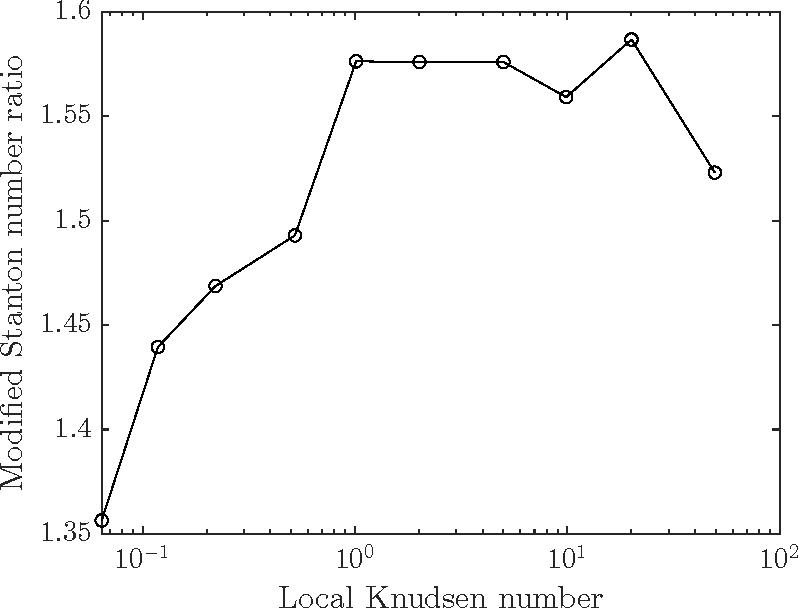
\includegraphics[width=0.52\textwidth]{Images/4. Results/Radius/stkn.pdf}
    \caption[Stanton number ratio vs local Knudsen number for the varying edge radius test case.]{Stanton number ratio vs local Knudsen number for the varying edge radius test case. Note that the datapoints included are the ones from the test cases in \autoref{fig:radiusstsec}.}
    \label{fig:radiusstkn}
\end{figure}

The second section of the graph also gives some relevant insight: as the Stanton ratio does not increase or decrease with local Knudsen number, the change observed in \autoref{fig:ratiokn} could be only due to a change in global Knudsen number.

\subsection{Constant local Knudsen number results}
\autoref{fig:localhtsec} and \autoref{fig:localstsec} respectively show the heat transfer and Stanton number distribution along the square contour for the constant local Knudsen number case. As shown in \autoref{tab:local}, a radius reduction corresponded to an equivalent Knudsen number increase, with the aim of maintaining the local Knudsen number constant. This objective was unfortunately not reached, as the theorised proportionality between local and global Knudsen numbers proved to not be valid.

Features noted when independently varying global Knudsen number and edge radius are both present, such as the more gentle decrease in heat transfer past the square corner or the order of magnitude increase in heat transfer. From \autoref{fig:localstsec} it is possible to note the presence of a Stanton number peak at the corner of the $Kn = 10$ case. Computing the local Knudsen number (equal to approximately \num{2e5}) reveals that this peak is probably caused by a very significant local rarefaction zone.

\autoref{fig:localstkn} shows the variation in Stanton number with local Knudsen number for the constant local Knudsen number case. The trend looks very similar to the one observed in \autoref{fig:ratiokn}.

\begin{figure}[H]
    \centering
    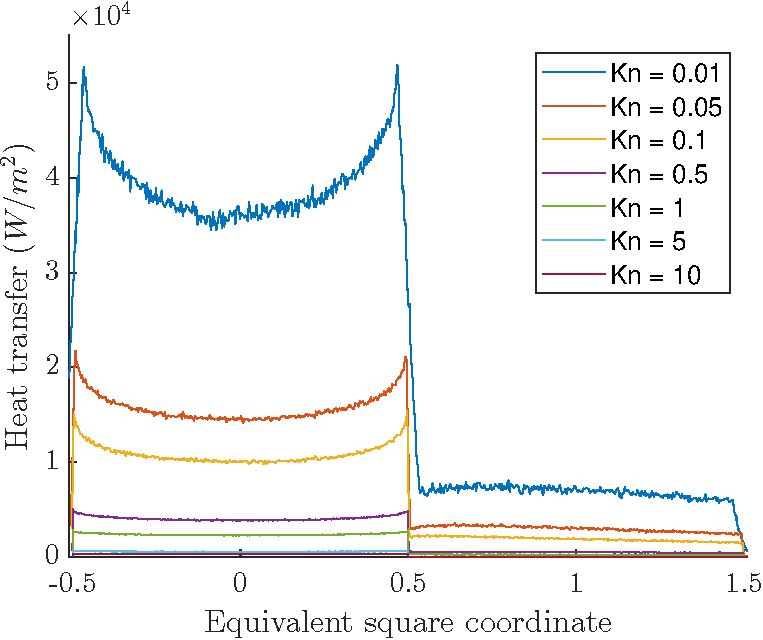
\includegraphics[width=0.52\textwidth]{Images/4. Results/local/htsec.pdf}
    \caption{Distribution of heat transfer along the square contour for constant local Knudsen number case.}
    \label{fig:localhtsec}
\end{figure}

\begin{figure}[H]
    \centering
    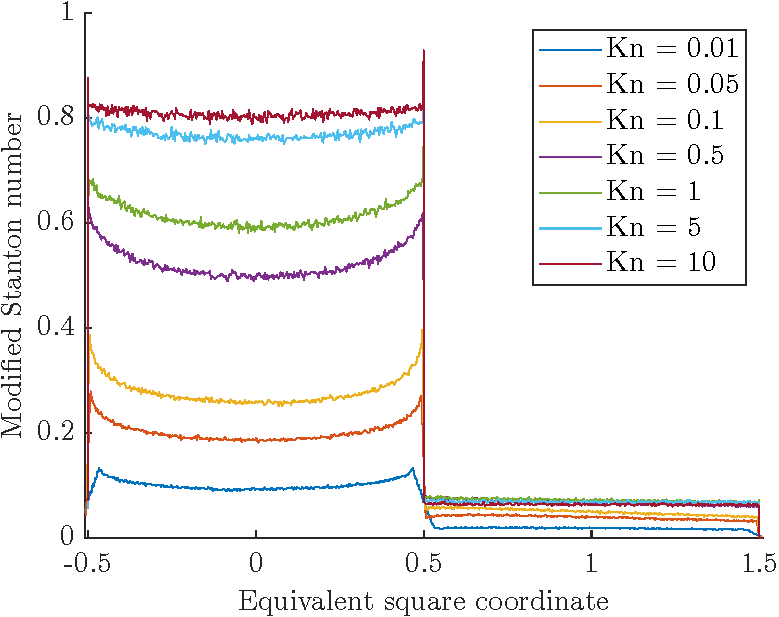
\includegraphics[width=0.52\textwidth]{Images/4. Results/local/stsec.pdf}
    \caption{Distribution of Stanton number along the square contour for constant local Knudsen number case.}
    \label{fig:localstsec}
\end{figure}

\begin{figure}[H]
    \centering
    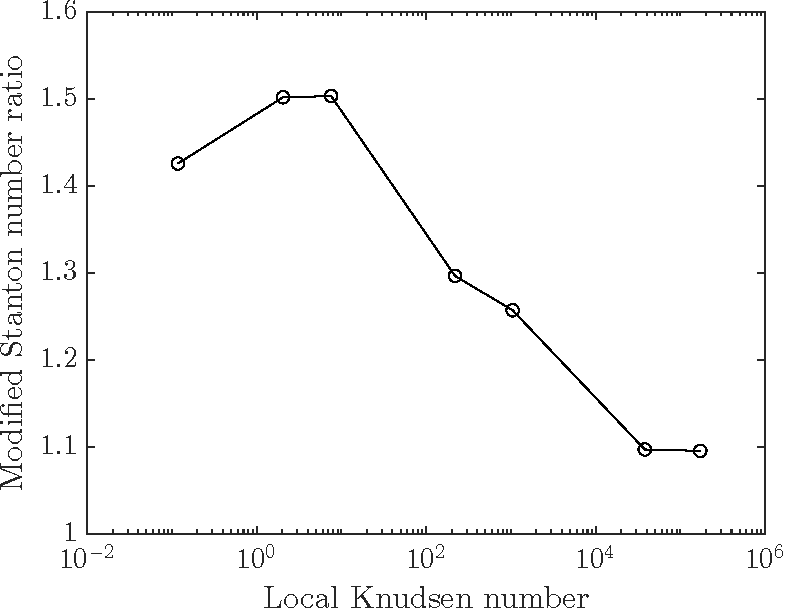
\includegraphics[width=0.52\textwidth]{Images/4. Results/local/stkn.pdf}
    \caption{Stanton number ratio vs local Knudsen number for constant local Knudsen number case.}
    \label{fig:localstkn}
\end{figure}

\subsection{Variation of angle of attack results}

\autoref{fig:aoa} shows the distribution of heat transfer along the square contour for varying values of angle of attack. As it is possible to see from it, the increase in heat transfer seen in literature \cite{pallahrini, spartavalid} has also been observed here.


\begin{figure}[H]
    \centering
    \begin{subfigure}{0.49\textwidth}
        \centering
        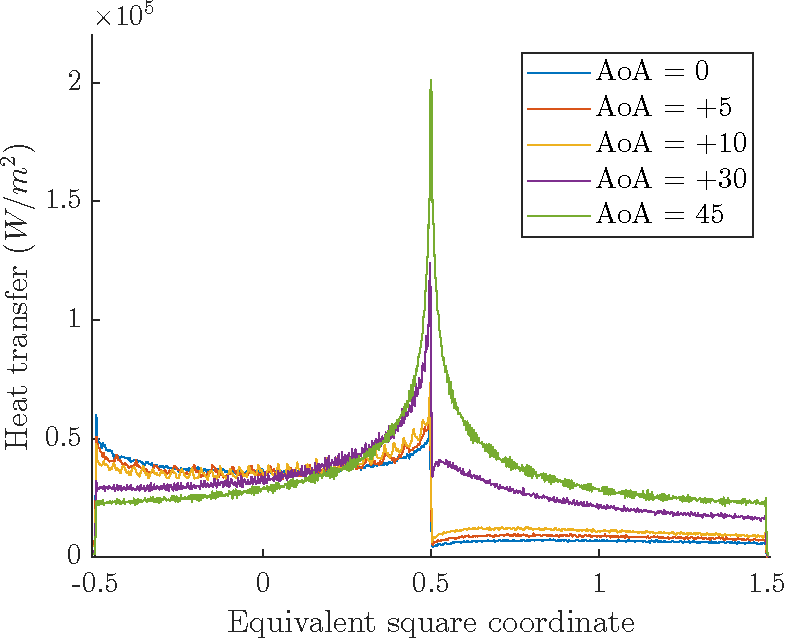
\includegraphics[width=\textwidth]{Images/4. Results/AoA/stsec+.pdf}
    \end{subfigure}
    \hfill
    \begin{subfigure}{0.49\textwidth}
        \centering
        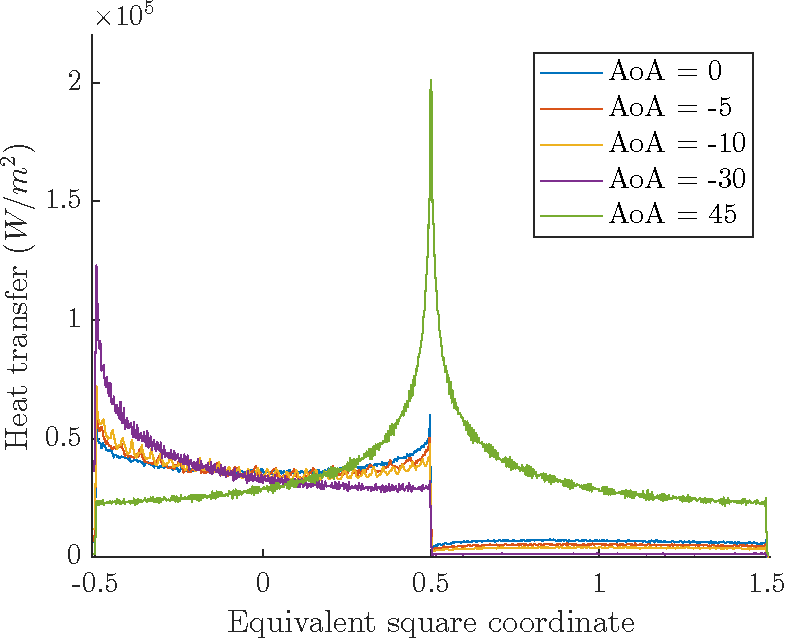
\includegraphics[width=\textwidth]{Images/4. Results/AoA/stsec-.pdf}
    \end{subfigure}
    \caption{Distribution of heat transfer along the square contour for varying values of angle of attack.}
    \label{fig:aoa}
\end{figure}

\subsection{Comparison of Stanton number ratio results}
\label{subsection:comparison}
The results obtained for the Stanton number variation with Knudsen number from the three test cases appear to be almost contradictory. The varying Knudsen number simulations show an explicit dependence on Knudsen number. This, coupled with the results of the varying radius simulations, which show an explicit independence of Stanton number with corner radius, would lead to believe that the change in Stanton number is only due to a change in density. However, if this was the case, the constant local Knudsen number simulation would have to only be dependent on global Knudsen number, and thus replicate the section of \autoref{fig:ratiokn} between the $Kn = 1$ and $Kn = 100$ (as the global Knudsen numbers of these datapoints match the ones used for the constant local Knudsen number simulations.

The decrease in ratio observed in \autoref{fig:ratiokn} and \autoref{fig:localstkn} is also of unknown origin. If it had been only observed in the varying Knudsen number case it could have probably been attributed to an unconverged mesh, as grid independence was not proven for a global Knudsen number of 0.001. However, the fact that this decrease has also been seen in the constant local Knudsen number case invalidates this theory, since the global Knudsen number for the first datapoint was equal to 0.01 (which was validated by mesh convergence)

Overall, this phenomenon appears to be quite complex, and further research is needed to identify a satisfactory correction factor to be implemented in rapid prototyping codes. This further research could be directed into modelling the lower Knudsen number regions through pure CFD or coupled DSMC-CFD codes, in order to provide some useful insight for the development of a valid correction factor.

\subsection{General considerations on the Direct Simulation Monte Carlo technique}
\label{subsection:dsmcdisc}
Direct Simulation Monte Carlo has overall proven to be a very useful and precise tool for the analysis of rarefied flows. Its computational cost prevents it however from leaving the academic setting, as powerful computing clusters are required for accurately simulating even very small domains: in the work carried out for this research thesis most of the simulations were run over multiple days on 40 state of the art server computing cores, despite the domain being limited to a 30 by \qty{30}{\cm} 2D square.
Employing this tool for full 3D simulations, larger domains or the modelling of the pure continuum regime remains thus still unfeasible, if not through the use of coupled DSMC-CFD codes or very powerful supercomputers.